\chapter{Wstęp}

Świat jest odwzorowywany przez programy komputerowe za pomocą modeli.
Zawierają one uproszczoną reprezentację rzeczywistości, a logika programu
umożliwia wykonywanie obliczeń na podstawie modelu, jego modyfikację, lub
utrwalenie i udostępnienie do wglądu innym osobom.
Modele te mogą być prezentowane użytkownikowi na wiele sposobów. Jednym z nich
jest reprezentacja graficzna w~formie diagramu. Taka metoda reprezentacji
ozwala użytkownikowi na łatwiejsze zrozumienie modelu
oraz jego modyfikację, w porównaniu do~formatu tekstowego, ponieważ jest
wizualna i przestrzenna, a więc jest naturalniejszą formą dla mózgu człowieka.

Przykładem modeli z reprezentacją graficzną, które są zrozumiałe zarówno dla
człowieka, jak i maszyny, oraz
przydają się podczas wytwarzania oprogramowania, są modele korzystające
z~\gls{UML}~\cite{wikipedia-uml}. Przedstawiają
one strukturę klas w programie oraz zależności między klasami. Na ich podstawie
czytelnik może wysokopoziomowo zapoznać się~ze strukturą programu, a
odpowiednie narzędzia pozwolą wygenerować kod klas w danym języku
programowania, który może służyć jako początek do późniejszego rozwoju
aplikacji. Przykładowy model \gls{UML} został przedstawiony na
rysunku~\ref{rys:przykladowy-model-uml}.

\begin{figure}[!hb]
	\centering
	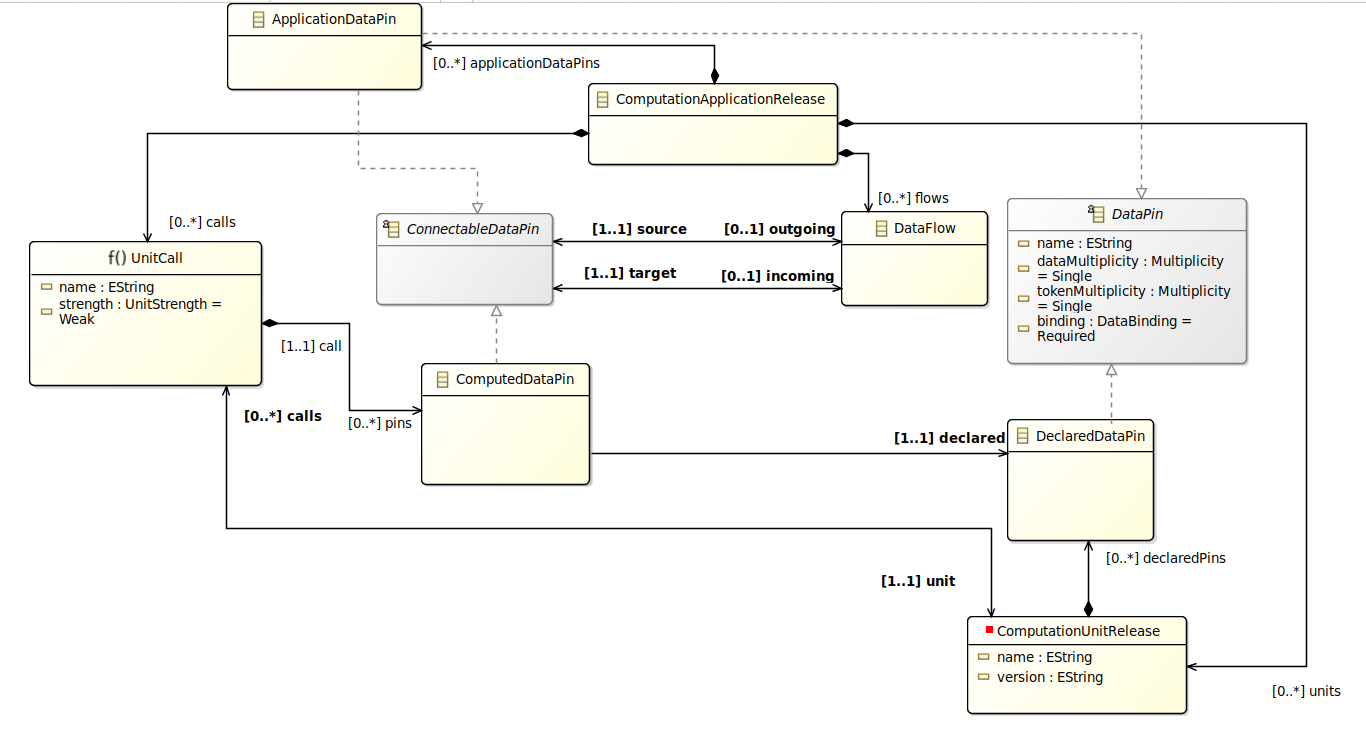
\includegraphics[width=0.95\linewidth]{./images/example-uml-model.png}
	\caption{Przykładowy model \gls{UML}.}\label{rys:przykladowy-model-uml}
\end{figure}

\gls{UML} jest przykładem uniwersalnego języka do opisu modeli klas programu.
Nie jest on~związany z żadną konkretną tematyką klas i pozwala na modelowanie
programów o~różnym zastosowaniu i przeznaczeniu. Istnieją także języki do opisu
modeli ściślej związanych z~konkretną dziedziną, czyli \gls{DSL}. Takie języki
są zazwyczaj mniejsze i mniej skomplikowane od języków uniwersalnych, a także
mają dokładniejszą semantykę (znaczenie elementów modelu). Potrafią więc one
odwzorować rzeczywistość w~sposób bardziej kompletny i zawrzeć więcej
szczegółów.

Strukturę samego modelu opisuje metamodel. Jest to model, który definiuje jakie
są~możliwe typy elementów modelu, jakie mają atrybuty, jak są połączone ze
sobą (składnia języka modelowania). Sam metamodel może być opisany na przykład
w języku UML\@ lub podobnym
bazowanym na nim, który będzie możliwiał wprowadzenie większej liczby
szczegółów. Taki metamodel często należy uzupełnić o zasady semantyczne ---
informacje o znaczeniu elementów, które nie mogą być zapisane w strukturze
metamodelu. Przykładową informacją semantyczną w modelu UML może być informacja
o krotności asocjacji.

\emph{BalticLSC} jest platformą do obliczeń rozproszonych wykonywaną z
inicjatywy
\emph{INTERREG Regionu Morza Bałtyckiego Unit Europejskiej}. Platforma ta
pozwala
wykonać obliczenia wykorzystując dostępne moduły obliczeniowe. Aplikacje
obliczeniowe definiowane są w postaci diagramów przedstawiających przepływ
danych między modułami obliczeniowymi. Przykład diagramu opisującego aplikację
obliczeniową został przedstawiony na
rysunku~\ref{rys:przykladowy-diagram-balticlsc}.  Model obliczeń opisany jest w
języku \gls{CAL}, który jest opisany za pomocą metamodelu~\cite{cal-metamodel}.

\begin{figure}[!hb]
	\centering

	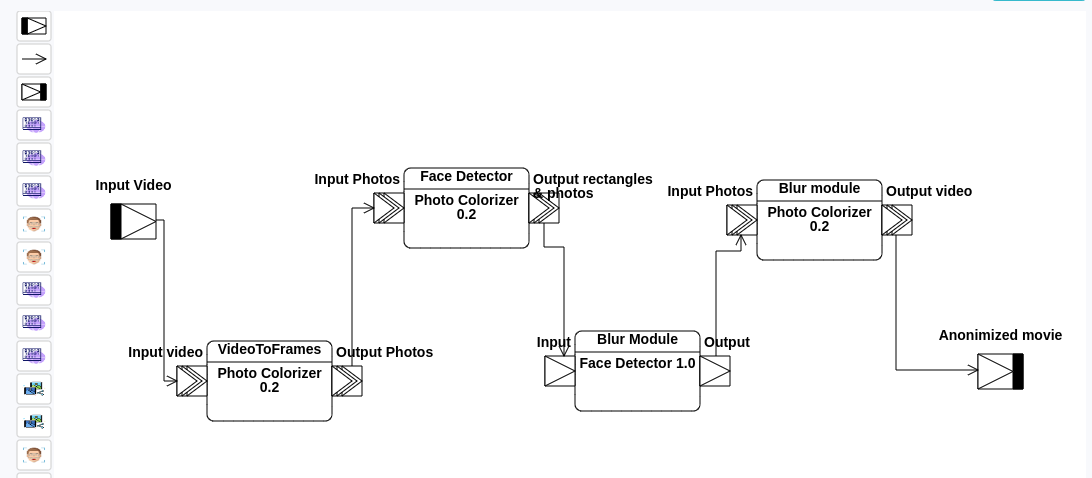
\includegraphics[width=0.95\linewidth]{./images/balticlsc-example-diagram.png}
	\caption{Przykładowy diagram przedstawiający aplikację obliczeniową w
		BalticLSC\@.}\label{rys:przykladowy-diagram-balticlsc}
\end{figure}

Istniejący edytor diagramów w BalticLSC dostępny jest jako część aplikacji
przeglądarkowej udostępnionej przez platformę. Do komunikacji z aplikacją
serwerową wykorzystuje inną reprezentację aplikacji obliczeniowej --- zapisuje
ją w postaci pudełek (prostokątów) oraz połączeń między nimi. Nie komunikuje
się on z aplikacją serwerową przesyłając informacje o strukturze modelu
zgodnej z metamodelem języka \gls{CAL}. Sprawia to, że po obu stronach (serwera
i aplikacji przeglądarkowej) potrzebne są dodatkowe transformacje
przetwarzające ogólny opis diagramu na model aplikacji obliczeniowej.

Sirius Web~\cite{sirius-web-github} jest narzędziem przygotowywanym przez firmę
Eclipse do tworzenia edytorów
diagramów działających w przeglądarce bazujących na metamodelach \gls{EMF}.
Technologia \gls{EMF} jest wykorzystywana od roku
2007~\cite{eclipse-sirius-wikipedia}, a metamodele
w~przeszłości mogły być tworzone używając oprogramowania Sirius
Desktop. Wykorzystując Sirius Web można w prosty sposób otrzymać aplikację
przeglądarkową umożliwiającą możliwości przeglądania i edycji modeli zbliżone
do tych,
które dotychczas oferowała jedynie aplikacja wymagająca instalacji na
komputerze użytkownika. Oprócz łatwiejszego dostępu do edytora diagramów dla
nowych użytkowników, wykorzystanie technologii przeglądarkowych do budowy
edytora diagramów pozwalają na dodanie mechanizmów kontroli dostępu do
wybranych modeli dla pewnych użytkowników, a także możliwości współpracy nad
modelem przez różne osoby w~czasie rzeczywistym.

W ustrukturyzowanym modelu zawierającym obiekty dziedzinowe w nietrudny sposób
można wyrazić reguły determinujące poprawność semantyczną modelu. Sirius
Desktop pozwala w tym zakresie na definiowanie semantycznych reguł
walidacyjnych, które są uruchamiane po każdej modyfikacji modelu i pokazują
błędnie umieszczone elementy. Odpowiednik tej funkcjonalności jest pożądany
także w edytorach diagramów opartych na Sirius Web.

W ramach tej pracy magisterskiej przygotowany został edytor diagramów dla
systemu BalticLSC korzystający z \emph{Sirius Web}. Edytor ten bazuje na
formalnym metamodelu \gls{EMF} opisującym język \gls{CAL} do
opisu aplikacji obliczeniowej. Ponadto, dostarczona została metoda sprawdzania
poprawności przygotowywanych przez użytkownika modeli na podstawie
zdefiniowanych reguł walidacji.

\section{Motywacja i cel pracy}

Jedną z alternatyw do wykorzystania Sirius Web do budowy edytora diagramów jest
wykorzystanie gotowych bibliotek JavaScript do wyświetlania i modyfikacji
diagramów (przykłady: \emph{react-diagrams}~\cite{react-diagrams-github},
\emph{Cytoscape.js}~\cite{cytoscape-js-homepage},
\emph{vis-network}~\cite{vis-network-github}). Są one ogólnymi narzędziami
pozwalającymi na zbudowanie własnego edytora diagramów. Dają sporą dowolność w
kwestii wyświetlania diagramu oraz
dostępnych funkcjonalności. Nie narzucają one
wykorzystania ustrukturyzowanych modeli poprzez wymaganie stworzenia
metamodelu. Z uwagi na swoją ogólność są trudniejsze do dostosowania do
własnych potrzeb, ponieważ funkcjonalności takie jak zapisywanie modeli w bazie
danych, współpraca w czasie rzeczywistym, walidacja modelu należy
zaimplementować samemu. Ponadto, modyfikacja takiego edytora diagramów wymaga
znajomości języka JavaScript.

Sirius Web dostarcza większość z tych
funkcjonalności wymagając jedynie wskazania metamodelu, który ma wykorzystywać.
Korzyści płynące z łatwego do przygotowania przeglądarkowego edytora diagramów
dla wybranych przez
nas modeli prezentują technologię Sirius Web jako interesującą i wartą użycia,
pomimo jej wczesnej fazy rozwoju i braku dokumentacji.

Celem tej pracy magisterskiej jest zbadanie możliwości udostępnianych przez
Sirius Web poprzez wykorzystanie go do przygotowania edytora
diagramów dla modeli języka CAL na platformie BalticLSC\@. Elementem edytora,
na który należy zwrócić szczególną uwagę, jest możliwosć walidacji modeli,
czyli weryfikacji ich~poprawności strukturalnej i semantycznej.

Ponadto, praca ta będzie jednym z pierwszych zastosowań Sirius Web wykonanych
przez osoby spoza zespołu budującego tą technologię, co może dostarczyć
dodatkowych informacji zwrotnych na temat prostoty jego wykorzystania, a także
napotkanych błędów i~niedociągnięć. Dla osób rozważających budowę edytora
modeli w oparciu o Sirius Web, praca ta będzie stanowiła źródło informacji o
wrażeniach z wykorzystania tej technologii, co pomoże podjąć bardziej świadomą
decyzję o używanych technologiach.
Z uwagi na brak dostępnej dokumentacji Sirius Web, praca ta może służyć również
jako przykład wykorzystania własnego metamodelu w tym edytorze diagramów.

Taki edytor diagramów bazujący na Sirius Web mógłby również zostać wykorzystany
w~aplikacji przeglądarkowej platformy BalticLSC\@. Jest on oparty o
ustrukturyzowany opis modelu, co pozwoliłoby na uproszczenie metody komunikacji
między serwerem aplikacyjnym a~aplikacją przeglądarkową, ponieważ nie byłyby
wymagane transformacje z aktualnego, ogólnego formatu danych do formatu
zgodnego z metamodelem.

\section{Zakres pracy}

W ramach pracy magisterskiej wykonano następujące czynności:

\begin{itemize}
	\item Stworzenie metamodelu języka \gls{CAL} w \gls{EMF}\@ z wykorzystaniem Sirius Desktop.
	\item Wykorzystanie tego metamodelu w Sirius Web. Zgłoszenie usterek autorom Sirius Web poprzez GitHub.
	\item Porównanie możliwości Sirius Web i Sirius Desktop. Zgłoszenie brakujących funkcjonalności autorom Sirius Web poprzez GitHub.
	\item Dodanie do metamodelu elementów usprawniających pracę z nim (automatyzacja niektórych czynności, dodanie ograniczeń utrudniających zrobienie błędu).
	\item Modyfikacja przeglądarkowego interfejsu użytkownika Sirius Web poprzez dodanie do niego przybornika z BalticLSC\@. Przybornik umożliwia w łatwy sposób dodanie nowych elementów do modelu.
	\item Dodanie mechanizmu walidacji semantycznej modelu sprawdzającego poprawność modelu z regułami zdefiniowanymi w języku Java.
	\item Stworzenie planu integracji rozwiązania z BalticLSC\@.
	\item Stworzenie przykładowej aplikacji przeglądarkowej zawierającej jedynie edytor diagramów z Sirius Web. Taki przykład pokazuje możliwość wykorzystania Sirius Web jako element innej aplikacji przeglądarkowej.
\end{itemize}

\vspace{1em}

\noindent Poza zakresem pracy pozostały następujące czynności:

\begin{itemize}
	\item Integracja stworzonego rozwiązania jako alternatywnego edytora diagramów dla systemu BalticLSC\@.
	\item Naprawa zgłoszonych usterek w Sirius Web.
\end{itemize}

\chapter{Tworzenie edytorów graficznych na bazie metamodeli}

Aplikacje komputerowe wykorzystują elementy graficzne aby ułatwić i
przyśpieszyć użytkownikom pracę.
Dzieje się to z uwagi na fakt, że ludzie bardziej efektywnie przyswajają
informacje wizualne (obrazki, diagramy), niż
tekst~\cite{images-more-effective-article}.
W przypadku użytkownika
wpływającego na~zachowanie systemu w sposób wizualny (np.\ edytując diagram),
korzysta on wtedy z~edytora graficznego i modyfikuje pewien model
rzeczywistości reprezentowany przez program. Model ten zaprojektowany jest
przez twórcę aplikacji i jego struktura również może być~reprezentowana na
wiele sposobów. Jeżeli struktura modelu sama jest opisywana przez model (o
wyższym poziomie abstrakcji) to mówimy, że~ten model modelu to
\emph{metamodel}.

\section{Metamodelowanie}

\emph{Metamodelowanie} w kontekście wytwarzania oprogramowania to
technika polegająca
na~przygotowaniu abstrakcyjnego modelu (metamodelu) opisującego strukturę
modeli, które będą wykorzystywane w programie. Metamodel określa jakie są
dopuszczalne typy obiektów w~modelu, ich atrybuty, powiązania między nimi.
Definiuje składnię języka projektowania. Przedrostek \emph{meta} oznacza, że
poziom abstrakcji tego metamodelu jest wyższy niż poziom abstrakcji modelu,
który opisuje~\cite{from-requirements-to-java-in-a-snap}.

W rodzinie metamodeli przestrzenią o najmniejszym poziomie abstrakcji jest
świat rzeczywisty (przestrzeń \emph{M0}). W programach komputerowych będzie on
reprezentowany przez model, który znajduje się w przestrzeni o wyższym poziomie
abstrakcji, \emph{M1}. Idąc dalej, modele będą oparte na metamodelach dla danej
dziedziny, które znajdują się w przestrzeni \emph{M2}. One~z~kolei są oparte na
meta--metamodelach % chktex 8
z przestrzeni \emph{M3}, które mają najwyższy poziom
abstrakcji w tej rodzinie. \emphgls{MOF}~\cite{mof-omg-specification} jest
przykładem meta--metamodelu. % chktex 8
Jest~zdefiniowany za pomocą samego siebie.

% TODO: dodać referencję z bibliografii

Wiele powszechnie znanych języków projektowania diagramów ma swoje metamodele
definiujące ich strukturę:

\begin{itemize}
	\item \emphgls{UML} ma swoją specyfikację~\cite{uml-omg-specification}
	      i metamodel opisany w języku \emphgls{MOF}.

	\item \emphgls{BPMN} (język do opisu procesów biznesowych) ma swój
	      metamodel~\cite{bpmn-omg-specification} również opisany w języku \emphgls{MOF}.

	\item Istnieje artykuł proponujący metamodel dla \emphgls{ERM}~\cite{entity-relationship-metamodel}. Dla~przypomnienia, \emphgls{ERM} pozwala przedstawić na diagramie encje bazy danych i~powiązania między nimi.
\end{itemize}

W metamodelu zdefiniowana jest składnia abstrakcyjna modelu, czyli struktura
jego elementów, oraz składnia konkretna, czyli jak one mają być reprezentowane,
na przykład na~diagramie.
Aby model był funkcjonalny oprócz jego struktury (składni języka projektowania)
należy zdefiniować i przestrzegać jego semantyki. To ona decyduje o tym jak
należy interpretować model, a także jakie sytuacje, pomimo bycia poprawnymi
strukturalnie, byłyby niewłaściwe z~punktu widzenia ich sensowności.

Przykładowo, w języku \emphgls{UML} z perspektywy struktury możliwe jest
utworzenie dwóch klas i dwóch połączeń kompozycji między nimi, co zostało
zademonstrowane na rysunku~\ref{rys:nieprawidlowy-model-uml}. Taki model jest
semantycznie niepoprawny, ponieważ relacja kompozycji oznacza, że jeden obiekt
jest zawarty w drugim obiekcie. Oznaczałoby to, że zarówno osoba
(\emph{Person}) jest zawarta w obiekcie samochodu (\emph{Car}) jako jego
właściciel, jak i samochody są zawarte w obiekcie właściciela.

\begin{figure}[!hb]
	\centering

	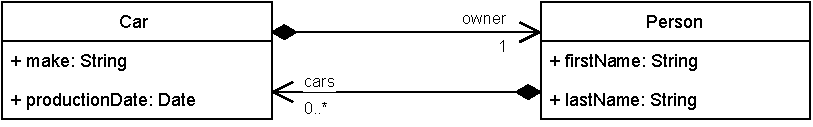
\includegraphics[width=0.95\linewidth]{./images/invalid-uml-example.pdf}
	\caption{Przykład modelu \emphgls{UML} nieprawidłowego
		semantycznie}\label{rys:nieprawidlowy-model-uml}
\end{figure}

Dopiero znając znaczenie relacji kompozycji można zauważyć ten błąd semantyczny
i~go~poprawić, na przykład jak na rysunku~\ref{rys:prawidlowy-model-uml}. Na
tym diagramie to osoba (\emph{Person}) jest obiektem nadrzędnym, który może
zawierać w sobie odniesienia do samochodów (\emph{Car}). Taki diagram jest
poprawny zarówno składniowo, jak i semantycznie.

\begin{figure}[!hb]
	\centering

	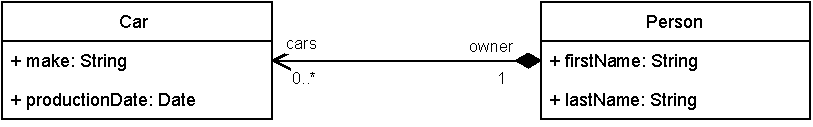
\includegraphics[width=0.95\linewidth]{./images/valid-uml-example.pdf}
	\caption{Przykład prawidłowego modelu
		\emphgls{UML}}\label{rys:prawidlowy-model-uml}
\end{figure}

\section{Edytory graficzne na podstawie metamodeli}

Metamodele mogą być zapisane w formacie, który jest przyjazny do odczytu
maszynowego. Oznacza to, że narzędzia będą mogły go odczytać, zinterpretować, a
także edytować. Sam~metamodel może mieć swój meta-metamodel, który zdefiniuje
jego strukturę.

Taki sformalizowany sposób przechowywania metamodelu ma wiele
korzyści. Przede wszystkim metamodel może być wtedy projektowany i edytowany w
narzędziu umożliwiającym robienie tego w najprostszy dla użytkownika sposób, na
przykład poprzez reprezentację metamodelu jako diagram. Ponadto, narzędzia mogą
wygenerować kod w konkretnym języku programowania. Zawierać on może klasy lub
inne mechanizmy przedstawienia modelu w tym języku programowania oraz może
wspierać operacje takie jak edycja, sprawdzenie poprawności składniowej
modelu.

Skoro znana jest struktura modelu, a więc wszystkie możliwe elementy i ich
połączenia, możliwe jest stworzenie edytora modeli, który będzie oparty na
metamodelu. Otrzymanie edytora diagramów dla danej dziedziny odbywa się dzięki
temu niskim nakładem czasowym --- wystarczy zdefiniować metamodel dziedziny, a
także zdefiniować wygląd elementów. Wymaga to mniejszej ilości czasu i
umiejętności w porównaniu z budową edytora diagramów korzystając z
edytorów diagramów ogólnego zastosowania.

\begin{figure}[!b]
	\centering

	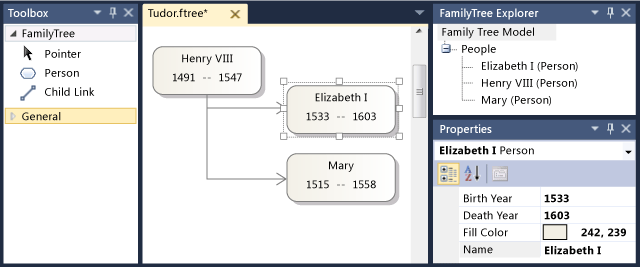
\includegraphics[width=0.95\linewidth]{./images/visual-studio-dsl-example.png}
	\caption{Edytowanie modelu w \emph{Visual Studio DSL
			Tools}}\label{rys:visual-studio-dsl-example}
\end{figure}

Przykładem zestawu narzędzi dostarczającego możliwości metamodelowania i
późniejszego generowania edytora graficznego dla modelu jest \emph{Visual
	Studio DSL Tools}~\cite{visual-studio-dsl-introduction} utworzone przez
firmę \emph{Microsoft}. Jest to zestaw
narzędzi do definiowania metamodelu, a następnie przygotowania rozszerzenia do
\emph{Visual Studio} w formacie \emphgls{VSIX}. Po jego zainstalowaniu
\emph{Visual Studio} nabiera możliwości graficznego edytowania modeli
bazujących na danym metamodelu. Edycja przykładowego modelu przedstawiona jest
na rysunku~\ref{rys:visual-studio-dsl-example}. Ponadto, tak przygotowany
edytor
może również generować klasy języka \emph{C\#} pozwalające na reprezentację
modelu, a
także jego serializację i deserializację. Dodatkową funkcjonalnością jest
również możliwość tworzenia plików na podstawie szablonów przygotowanych dla
metamodelu. W ten sposób można wygenerować na przykład tabelę w~języku
\emphgls{HTML} zawierającą wszystkie elementy konkretnego typu w modelu.

Innym narzędziem umożliwiającym przygotowanie edytora graficznego na podstawie
metamodelu jest \SiriusDesktop{}~\cite{sirius-desktop-homepage} rozwijany
przez firmę \Eclipse{}. Jest to rozszerzenie do~zintegrowanego środowiska
programistycznego (\emphgls{IDE}) \Eclipse{}. Pozwala ono na zaprojektowanie
metamodelu dla wybranej dziedziny używając technologii \emph{\acrfull{EMF}}.
Jest on wyrażony za pomocą
meta--metamodelu  % chktex 8
\Ecore{} (rozszerzenie \texttt{*.ecore}) i jest
zapisany w pliku \emphgls{XML}. Interfejs użytkownika programu \SiriusDesktop{}
widoczny jest na rysunku~\ref{rys:sirius-desktop-example-metamodel}. Po lewej
dostępne jest drzewo metaklas, na środku widać diagram struktury struktury
metamodelu, a po prawej stronie znajduje się przybornik z~narzędziami do
tworzenia elementów metamodelu. W \SiriusDesktop{}
można wygenerować 5 pakietów opisanych w kolejnych akapitach.

\begin{figure}[!ht]
	\centering

	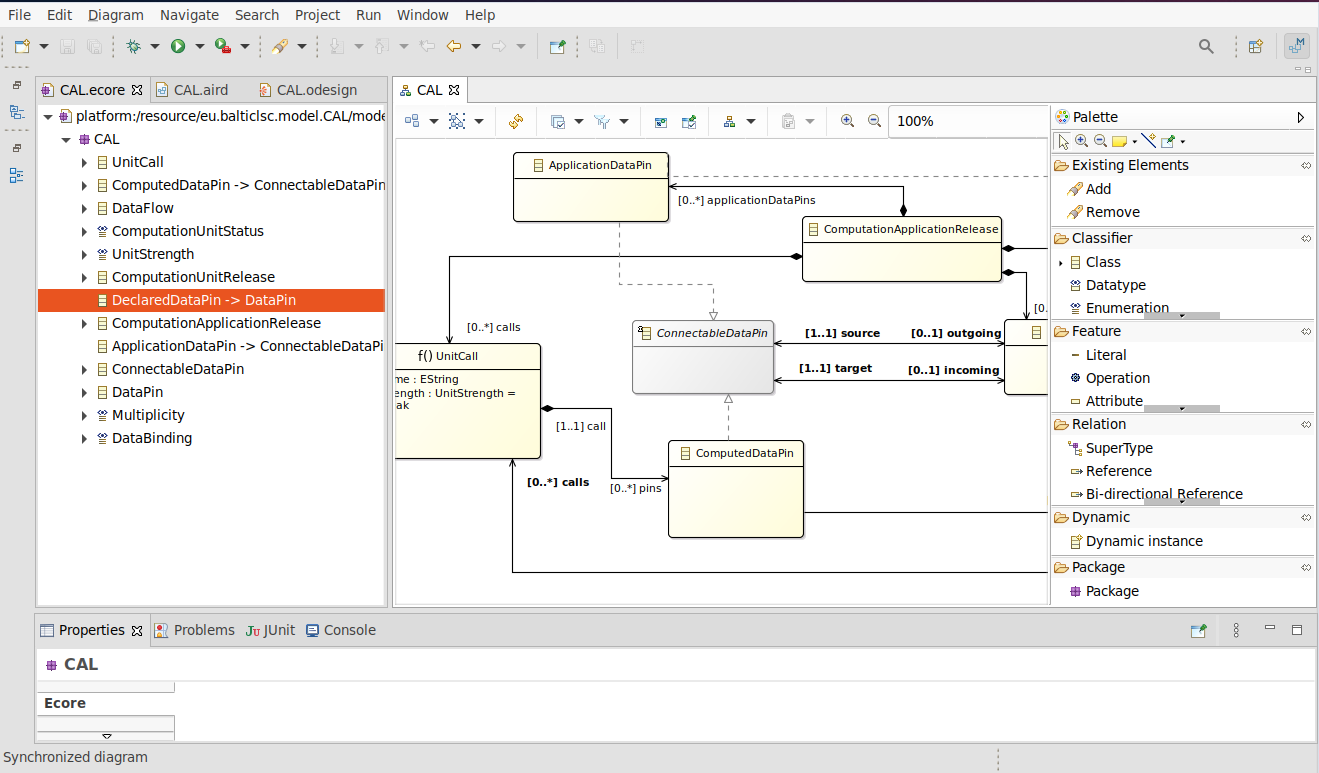
\includegraphics[width=0.95\linewidth]{./images/sirius-desktop-metamodel.png}
	\caption{Projektowanie metamodelu w \emph{Sirius
			Desktop}}\label{rys:sirius-desktop-example-metamodel}
\end{figure}

Pierwszym pakietem jest pakiet bazowy zawierający klasy umożliwiające
reprezentację modeli w
kodzie języka \Java{}, ich serializację i deserializację. Każdy obiekt
metamodelu
odpowiada klasie języka \Java{}. Klasy te zawierają mechanizmy powiadamiana o
zmianach (ang.~\emph{\selectlanguage{english}change detection}).
Możliwa jest modyfikacja kodu tych klas, co zmienia zachowanie
modelu.

Drugim z pakietów jest pakiet \texttt{.design} z plikiem o rozszerzeniu
\texttt{*.odesign} zawierający opis reprezentacji graficznych modelu. Każdy
model może mieć wiele reprezentacji graficznych z~różnymi poziomami
szczegółowości.
Możliwe reprezentacje graficzne to diagram klas, diagram
sekwencji, tabela, drzewo~\cite{dokumentacja-sirius-desktop}. Dla każdej
reprezentacji należy zdefiniować jak elementy modelu mają być wyświetlane.

Funkcjonalności ulepszające doświadczenia użytkownika z
korzystania z edytora zawierają także możliwość ustalenia styli warunkowych
(zmiany wyglądu elementu gdy spełnione zostaną ustalone warunki), zdefiniowanie
narzędzi pomagających w edycji diagramu (przykładowo okno dialogowe
wyświetlające formularz składający się z kilku kroków, który ostatecznie tworzy
kilka powiązanych ze sobą obiektów w modelu, albo narzędzie do kaskadowego
usuwania powiązanych elementów modelu), jak i możliwość opisania reguł
walidacji semantycznej, które będą uruchamiane po każdej zmianie i będą mogły
oznaczyć niepoprawne elementy modelu oraz zaproponować automatyczne ich
naprawienie.

Operacje wymagające wykonania dynamicznej logiki mogą być wprowadzone na 2
sposoby: poprzez napisanie kodu w języku \Java{} i udostępnienie go jako usługa
dostępna w~metamodelu, lub poprzez napisanie wyrażenia w języku
\emphgls{AQL}~\cite{dokumentacja-aql}.
Pozwala on~na~wybranie elementów z modelu (także podzbioru elementów
spełniających pewne kryteria), ich~atrybutów, oraz wykonanie operacji
logicznych na nich, na przykład ich~porównanie.

Trzecim pakietem jest pakiet \texttt{.edit}. Składa się on z klas
umożliwiających programatyczne odczytanie informacji o strukturze modelu ---
klasy zawierają opis właściwości obiektów modelu.

Czwartym pakietem jest pakiet \texttt{.editor}. Zawiera on definicję wtyczki do
środowiska \Eclipse{}, która dostarcza możliwości tworzenia i edycji
modeli. To właśnie ten pakiet umożliwia użycie wszystkich pozostałych pakietów
przez użytkownika i ostatecznie otrzymanie edytora graficznego. Edytor
diagramów dla przykładowego modelu został zaprezentowany na
rysunku~\ref{rys:sirius-desktop-example-model}.

\begin{figure}[!ht]
	\centering

	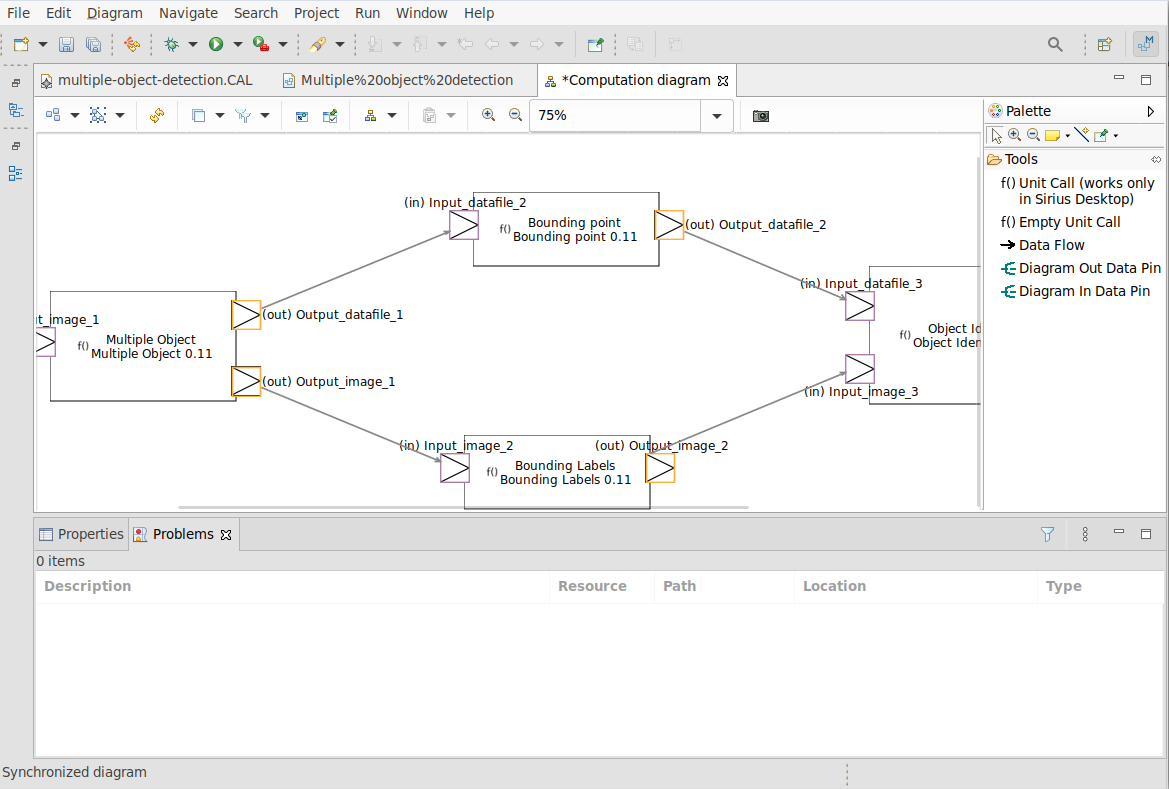
\includegraphics[width=0.95\linewidth]
	{./images/sirius-desktop-model-editor.png}
	\caption{Edycja przykładowego modelu w
		\SiriusDesktop{}}\label{rys:sirius-desktop-example-model}
\end{figure}

Piątym pakietem jest pakiet \texttt{.tests}. Można w nim tworzyć testy
zachowania metamodelu korzystając z środowiska uruchomieniowego do testów
\JUnit{}. Testy te przydają się~gdy~domyślne zachowanie modelu zostanie
zmodyfikowane poprzez edycję klas bazowych modelu w~głównym pakiecie projektu.

Edytor graficzny otrzymany dzięki pakietowi \texttt{.editor} jest wtyczką do
środowiska \Eclipse{}, które jest aplikacją systemową wymagającą instalacji
w systemie użytkownika zanim będzie on~mógł przeglądać i edytować modele.
Od 2018 roku~\cite{sirius-components-repo-first-commit} firma \Eclipse{}
pracuje nad~rozwiązaniem \SiriusWeb{}~\cite{sirius-web-github}, którego
celem jest przeniesienie edytora
graficznego dotychczas dostępnego w aplikacji natywnej do przeglądarki
internetowej. Interfejs użytkownika tego projektu jest widoczny na
rysunku~\ref{rys:sirius-web-ui}.

\begin{figure}[!ht]
	\centering

	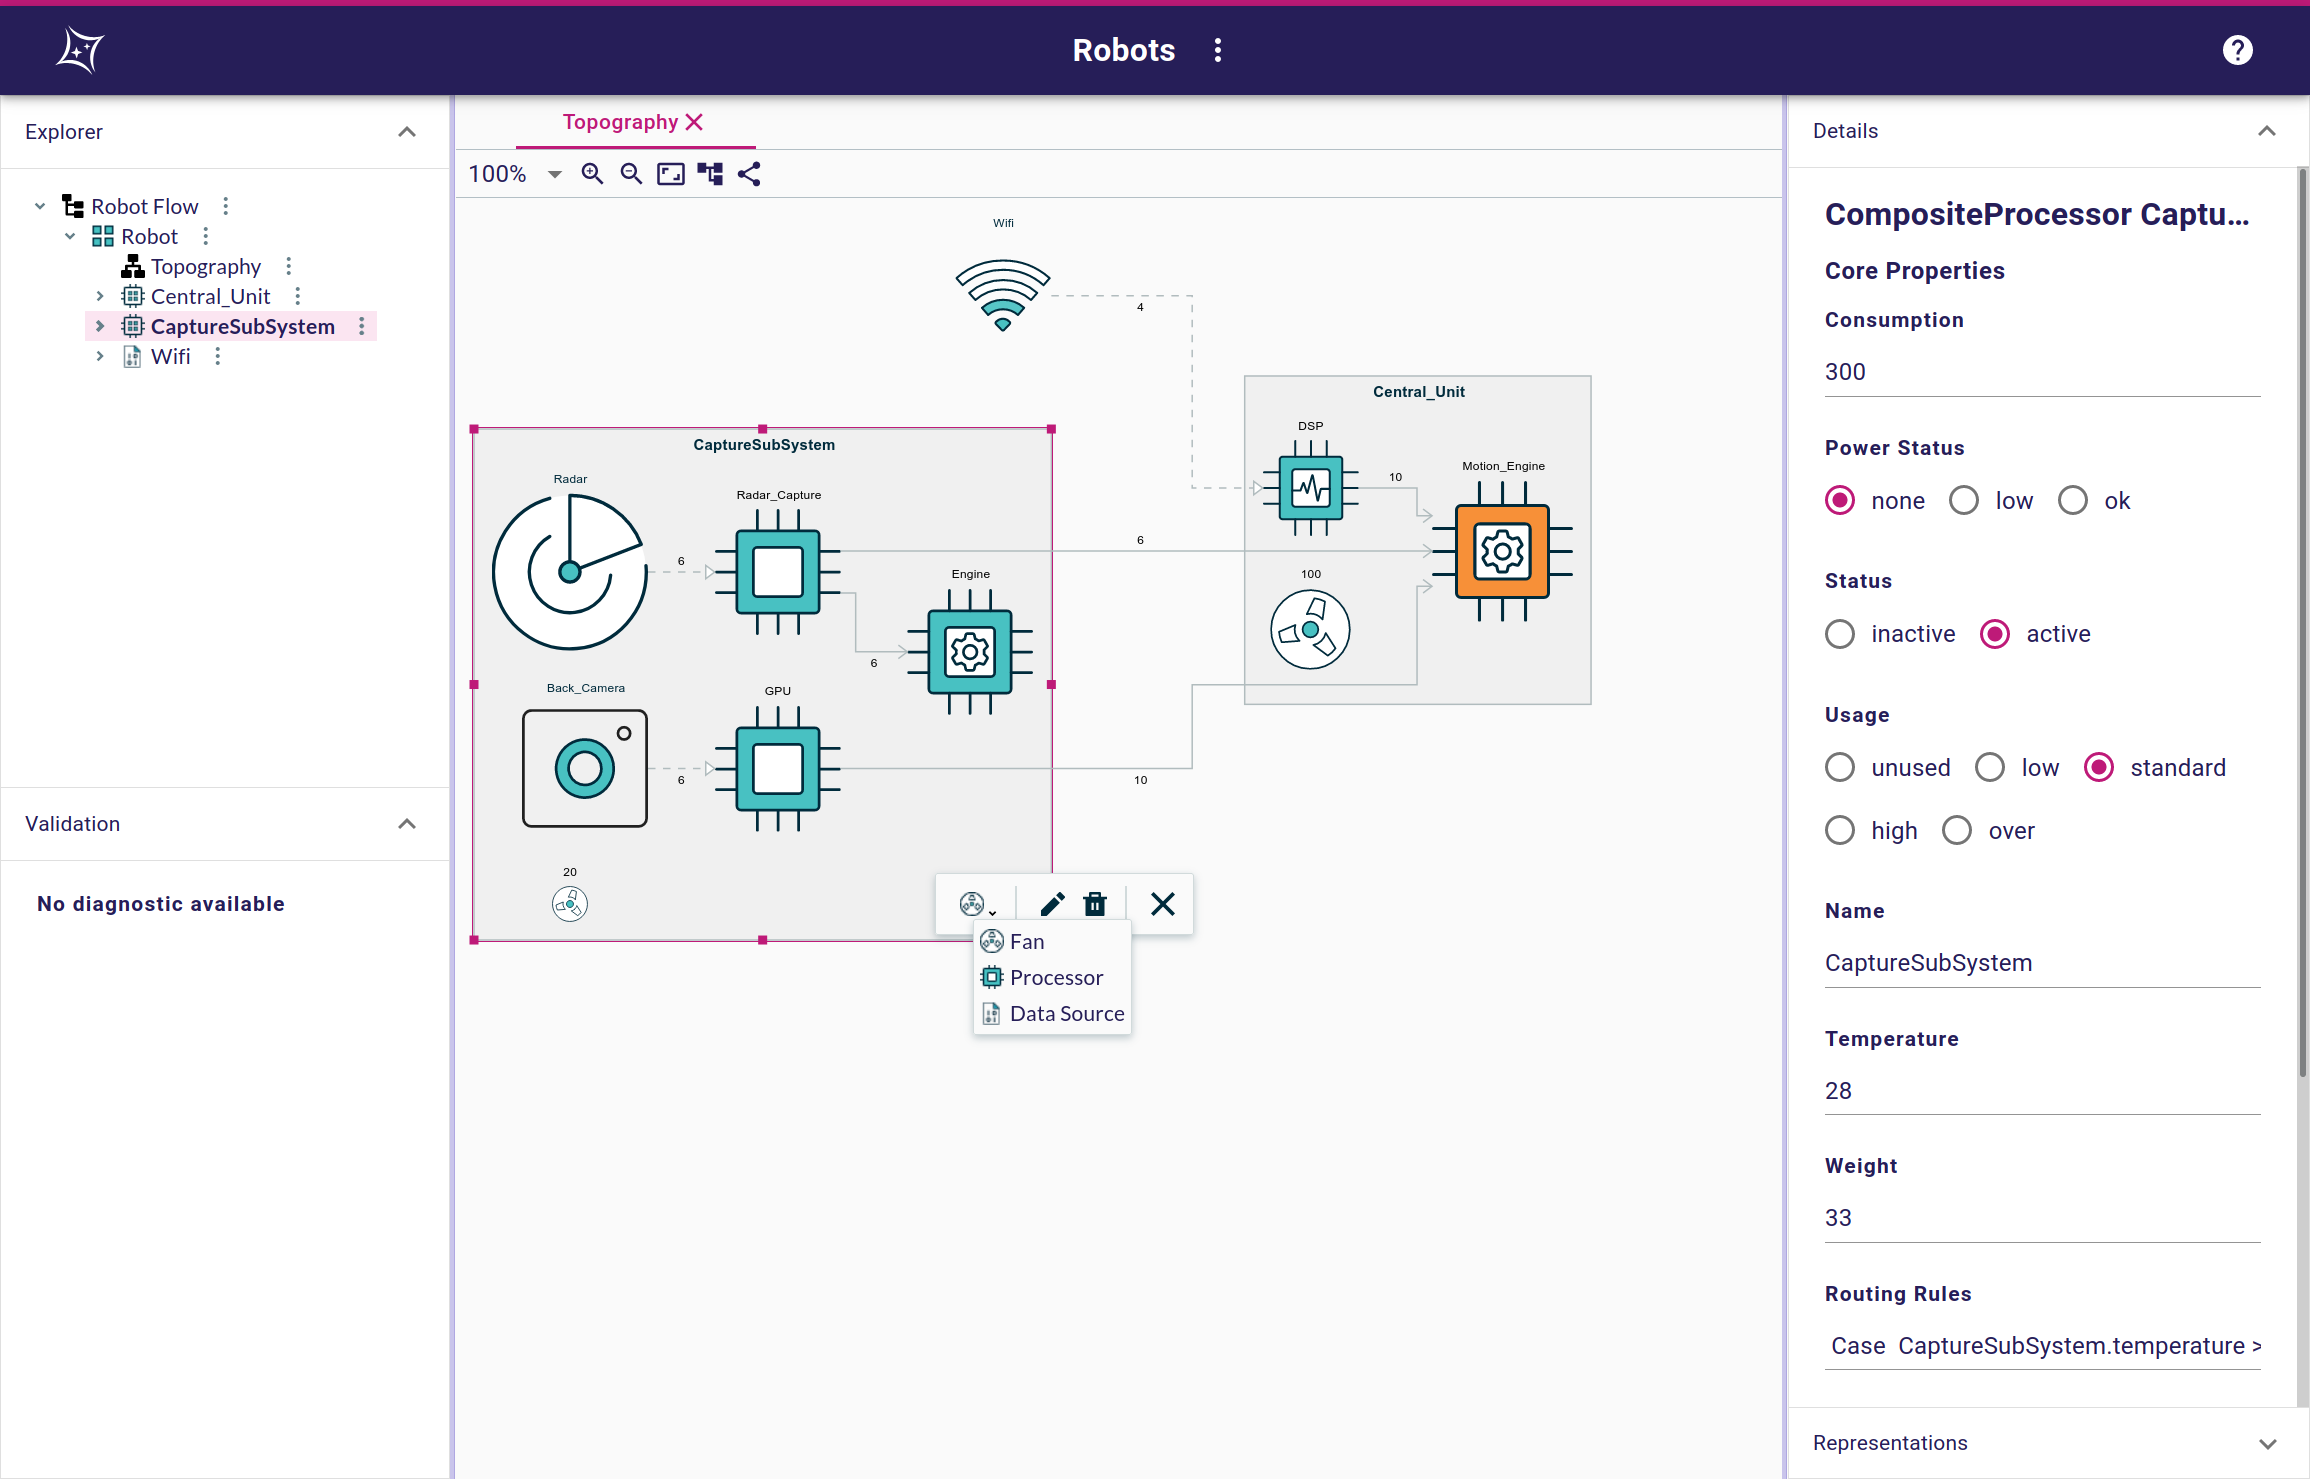
\includegraphics[width=0.95\linewidth]
	{./images/sirius-web-editor.png}
	\caption{Edytor modeli \SiriusWeb{}}\label{rys:sirius-web-ui}
	{\small Źródło: \url{https://github.com/eclipse-sirius/sirius-web}}
\end{figure}

\SiriusWeb{} składa się z 3 komponentów:

\begin{itemize}
	\item serwera aplikacyjnego stworzonego w technologii \emph{Java
		      Spring}~\cite{java-spring-homepage} dostarczającego interfejsu sieciowego \emphgls{API} w formacie \GraphQL{} pozwalającego na wyświetlenie oraz modyfikację modelu,
	\item bazy danych \PostgreSQL{}~\cite{postgresql-homepage} przechowującej informacje o modelach i użytkownikach,
	\item aplikacji przeglądarkowej napisanej z wykorzystaniem biblioteki \React{}~\cite{react-homepage} umożliwiającej wyświetlenie i modyfikację modeli w formie drzewa obiektów lub diagramu.
\end{itemize}

Metamodele, na których bazuje \SiriusWeb{} są w tym samym formacie \Ecore{} co
metamodele w \SiriusDesktop{}. Można zatem w łatwy sposób stworzyć
graficzny edytor modeli zarówno w~formie aplikacji natywnej, jak i
przeglądarkowej. Posiadając istniejący metamodel języka użyty
w~\SiriusDesktop{} można go w krótkim czasie przenieść do \SiriusWeb{}. Jest
to~możliwe, ponieważ serwer aplikacyjny korzysta z tych samych bibliotek i
pakietów do obsługi metamodelu, które są wykorzystywane w edytorze
\SiriusDesktop{}.

Zmianie uległ natomiast sposób przechowywania modeli. W \SiriusDesktop{}
były one~zapisane w plikach na dysku użytkownika. W \SiriusWeb{} są one
przechowywane w bazie danych \PostgreSQL{}. Taki format zapisu pozwala na
równoczesny dostęp do modelu przez wielu użytkowników i natychmiastowe
przesyłanie informacji o zmianach w czasie rzeczywistym dzięki użyciu
\emph{GraphQL Subscriptions}~\cite{graphql-subscriptions} (dwukierunkowych
połączeń do przesyłania ustrukturyzowanych danych między przeglądarką a
serwerem opartych na protokole \WebSocket{}~\cite{wikipedia-websocket}).
Oznacza to, że użytkownicy mogą w czasie rzeczywistym wspólnie edytować modele
i~natychmiast widzieć zmiany wprowadzone przez innych użytkowników.
Poprzez zgrupowanie modeli w~projekty wewnątrz aplikacji \SiriusWeb{}
możliwa jest również kontrola dostępu do nich --- administrator może określić
zasady dostępu użytkowników do poszczególnych projektów.

Udostępnienie edytora modeli jako aplikacja przeglądarkowa sprawia też, że jest
on~bardziej dostępny dla użytkowników. Mogą oni przeglądać i edytować modele
bez instalacji aplikacji natywnych w ich systemie --- wystarczy przeglądarka
internetowa, która jest zainstalowana na większości komputerów konsumenckich.
Można też w łatwiejszy sposób podzielić się~przygotowanym przez nas modelem,
ponieważ wystarczy wysłać adres \emphgls{URL} innemu użytkownikowi zamiast
wysyłać plik z modelem.

Poza tym łatwiejsze wprowadzanie jest poprawek i zmian do metamodelu.
W przypadku aplikacji natywnych i dzieleniu się modelem przechowywanym w pliku
należało zaktualizować metamodel oraz wszystkie jego modele, a później wysłać
nowe pliki modeli oraz nowy edytor wszystkim użytkownikom. Problemy powstają
gdy użytkownicy zmodyfikowali swoje modele przechowywane lokalnie i nie są już
one kompatybilne z nowym metamodelem, lub gdy użytkownicy przypadkowo używają
starego modelu przy pracy z modelami. Takie rozwiązanie zwiększa liczbę
możliwości na popełnienie błędu. W przypadku aplikacji internetowej wszyscy
pracują z~tymi samymi modelami przechowywanymi na serwerze. Osoby
odpowiedzialne za~metamodel mogą go zmodyfikować wraz z modelami zapisanymi w
bazie danych. Uruchomienie serwera z~nowym metamodelem wystarcza, aby wszyscy
użytkownicy po~otworzeniu edytora \SiriusWeb{} mieli jego najnowszą
wersję.


\chapter{Metamodel dla języka CAL}\label{chapter:cal-metamodel}

Aby otrzymać graficzny edytor modeli wykorzystując \emph{Sirius Web} należy
najpierw zaprojektować metamodel \gls{EMF} opisujący strukturę modeli oraz ich
reprezentację graficzną, która później będzie możliwa do modyfikacji przez
użytkowników. W tym rozdziale
zostanie omówiony język \acrfull{CAL} służący do opisu obliczeń w systemie
\emph{BalticLSC}, a~następnie omówiony zostanie przygotowany metamodel
\gls{EMF}.

\section{Język opisu obliczeń w BalticLSC}

Obliczenia rozproszone wykonywane przez system \emph{BalticLSC} są zapisywane w
formie \emph{aplikacji obliczeniowej}
(\emph{\selectlanguage{english}computation application})
korzystajac ze składni języka \acrfull{CAL} przygotowanego dla tego właśnie
systemu.

Podstawowym obiektem, który wysyła (wyjście)
lub odbiera (wejście) dane, jest \emph{port}. Jest on reprezentowany za pomocą
ikony kwadratu ze strzałką skierowaną w prawą stronę. Aplikacja obliczeniowa
składa
się z modułów obliczeniowych posiadających swoje porty, portów samej aplikacji
obliczeniowej, oraz połączeń między tymi portami. Grot połączenia wskazuje
kierunek przepływu danych.
Porty aplikacji obliczeniowej są zaznaczone na
diagramie ikoną portu (strzałką skierowaną w prawo) z pogrubioną
jedną z krawędzi ikony --- lewą dla wejścia, prawą dla wyjścia.

Porty modułów oraz aplikacji obliczeniowych mają różne ikony, które
są ustalane na~podstawie ich właściwości. Są dwa kryteria wpływające na ikonę:

\begin{itemize}
	\item krotność danych, które obsługuje port (\emph{data
		      multiplicity}):  dla pojedynczego pliku będzie to~pojedyncza strzałka, a dla katalogu --- wiele strzałek,
	\item liczba pakietów przyjmowanych lub wysyłanych danych (\emph{token
		      multiplicity}, czy oczekuje pojedynczego zestawu danych wejściowych, czy moduł obsłuży kolejne zestawy danych wysyłane po chwili bez ponownego uruchomienia).
\end{itemize}

Moduł obliczeniowy rozpoczyna obliczenia dopiero gdy na każdym jego wejściu
znajdują się dane.

Przykładowe aplikacje obliczeniowe zostały przedstawione na
rysunkach~\ref{rys:sekwencyjna-aplikacja-obliczeniowa}
i~\ref{rys:mozliwa-do-zrownoleglenia-aplikacja-obliczeniowa}.
Pierwsza z nich (rysunek~\ref{rys:sekwencyjna-aplikacja-obliczeniowa}) jest
aplikacją, w której obliczenia mogą zostać wykonane
wyłącznie sekwencyjnie, ponieważ dane przepływają sekwencyjnie od wejścia
kolejno przez moduły nazwane \texttt{VideoToFrames}, \texttt{Face Detector},
\texttt{Blur Module}, \texttt{Blur module}, aż w końcu trafiają do wyjścia.
Inna jest struktura aplikacji na
rysunku~\ref{rys:mozliwa-do-zrownoleglenia-aplikacja-obliczeniowa}. Tam
przepływ danych rozdziela się~po~module obliczeniowym \texttt{Pdf page
	splitter} i obliczenie modułów \texttt{OCT Tesseract Tess 0.1} oraz
\texttt{OCR Tesseract LSTM 0.1} może zostać wykonane równolegle, być może
przez różne węzły obliczeniowe. Ich wyniki trafią później do modułu \texttt{Pdf
	data joiner 0.1} i przejdą dalej przez pozostałe moduły w sposób
sekwencyjny.

\begin{figure}[!ht]
	\centering

	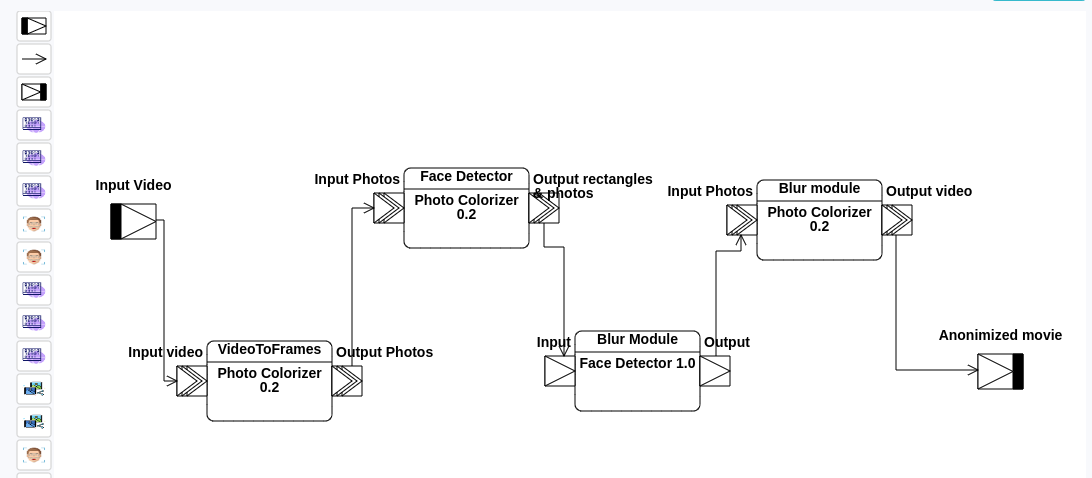
\includegraphics[width=0.95\linewidth]{./images/balticlsc-example-diagram.png}
	\caption{Aplikacja obliczeniowa w BalticLSC z obliczeniami
		sekwencyjnymi.}\label{rys:sekwencyjna-aplikacja-obliczeniowa}
\end{figure}

% \begin{noindent}
\begin{figure}[!ht]
	\centering

	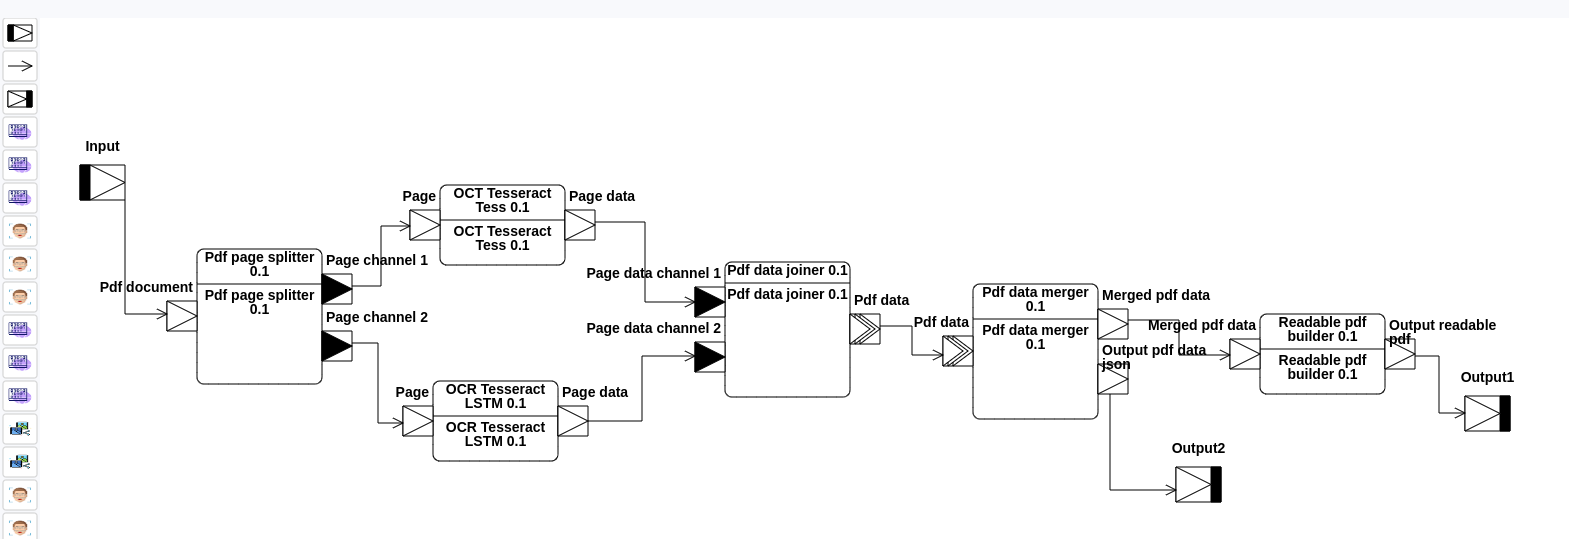
\includegraphics[width=0.99\linewidth]{./images/balticlsc-concurrent-application-example.png}
	\caption{Aplikacja obliczeniowa w BalticLSC z możliwością
		zrównoleglenia obliczeń.}\label{rys:mozliwa-do-zrownoleglenia-aplikacja-obliczeniowa}
\end{figure}
% \end{noindent}

\section{Stworzony metamodel EMF dla języka CAL}

Przygotowany metamodel \gls{EMF} dla języka \gls{CAL} widoczny jest na
rysunku~\ref{rys:cal-emf-metamodel}. Bazuje on~na metamodelu
opracowanym w ramach projektu BalticLSC~\cite{cal-metamodel}, który widoczny
jest na~rysunku~\ref{rys:cal-metamodel-balticlsc}.
Na potrzeby edytora diagramów nie są potrzebne wszystkie elementy oryginalnego
metamodelu. Niektóre klasy i właściwości zostały pominięte, ponieważ nie były
istotne z~perspektywy edycji diagramu.

\begin{figure}[!hb]
	\centering

	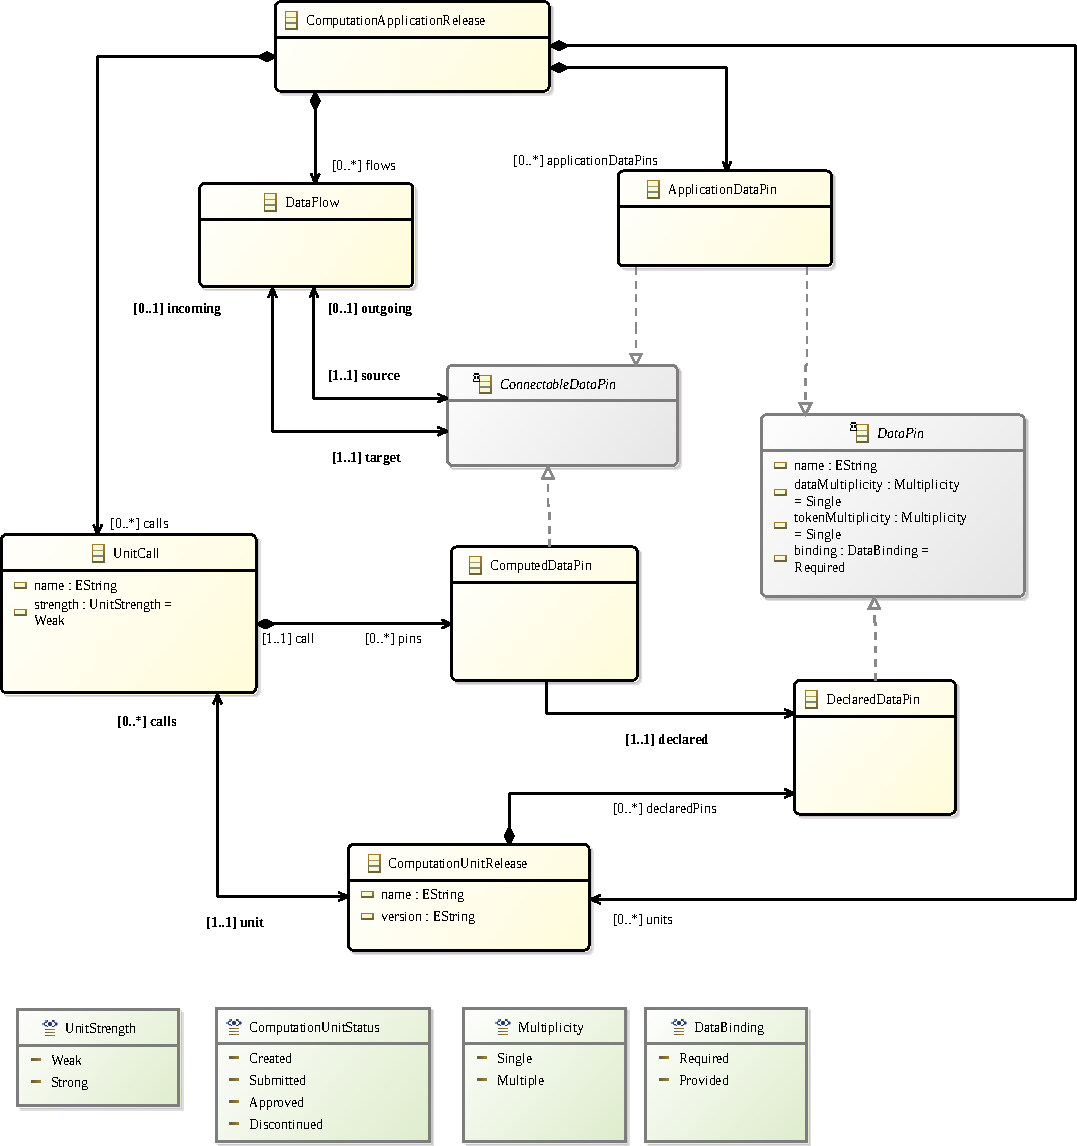
\includegraphics[width=0.92\linewidth]{./images/cal-emf-metamodel.pdf}
	\caption{Metamodel EMF języka CAL przygotowany w ramach tej
		pracy.}\label{rys:cal-emf-metamodel}
\end{figure}

\begin{figure}[!hb]
	\centering

	% NOTE: this image is pretty tall, so it must be kept much smaller than the
	% line width so it does not take up the whole page, moving all incoming
	% images to the bottom of the chapter.

	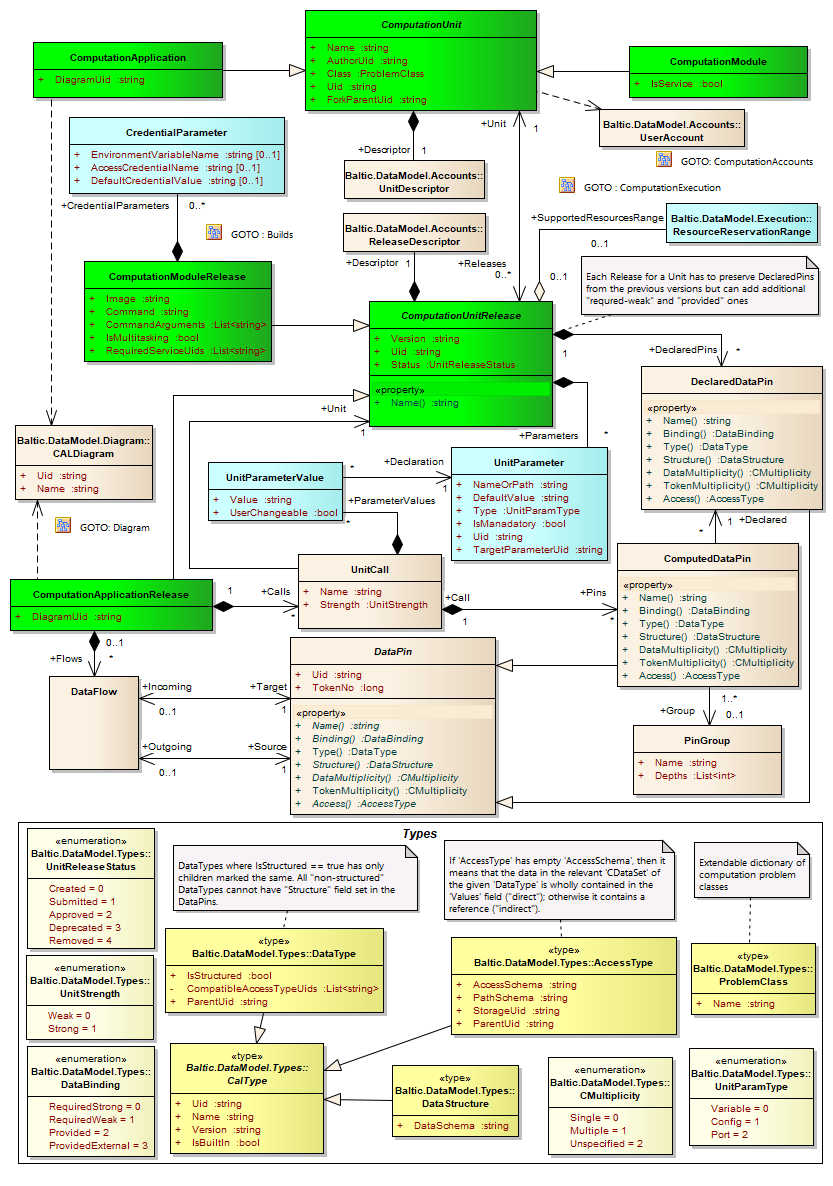
\includegraphics[width=0.82\linewidth]{./images/cal-metamodel-balticlsc.png}
	\caption{Metamodel języka CAL używany w projekcie
		BalticLSC\@.}\label{rys:cal-metamodel-balticlsc}

	\medskip
	{\small Źródło:
		\url{https://www.balticlsc.eu/model/index.htm?goto=4:2:404}}
\end{figure}

Model w EMF ma strukturę drzewiastą. Korzeniem drzewa jest obiekt typu
\texttt{ComputationApplicationRelease}, ktory odpowiada całemu diagramowi
(aplikacji obliczeniowej). Nie
ma on~własnych właściwości. Zawiera on w sobie natomiast 4 typy obiektów:

\begin{itemize}
	\item \texttt{ComputationUnitRelease} --- są to obiekty odpowiadające
	      rodzajom modułów obliczeniowych dostępnych w systemie BalticLSC i opisują ich właściwości.

	      Oprócz informacji o nazwie i wersji modułu zawierają w sobie obiekty \texttt{DeclaredDataPin} dziedziczące z \texttt{DataPin}, które opisują porty tego modułu obliczeniowego.

	      Obiekty te nie są wyświetlane na diagramie (nie występują w wizualnej reprezentacji modelu). Można je zobaczyć jedynie w drzewie obiektów modelu.

	\item \texttt{UnitCall} --- wywołania dostępnych modułów
	      obliczeniowych. Każdy dostępny moduł obliczeniowy może zostać wywołany dowolną liczbę razy. Każde wywołanie to osobny obiekt \texttt{UnitCall} ze wskazaniem modułu, który ma zostać wywołany, a także z obiektami \texttt{ComputedDataPin}, które reprezentują porty tego modułu.

	      Taka reprezentacja pozwala na zapisanie szczegółów dotyczących dostępnych modułow obliczeniowych wyłącznie raz w modelu, a później wskazywanie tych elementów w~każdym z wywołań modułu.

	      Rozwiązanie to ma jednak pewne ograniczenie --- aby oznaczyć wywołanie modułu za~pomocą obiektu \texttt{UnitCall}, należy najpierw stworzyć obiekt \texttt{ComputationUnitRelease} i~dodać odpowiednie \texttt{DeclaredDataPin}. Można wywołać jedynie moduły, które są~zapisane w metamodelu. Sam metamodel nie ma możliwości pobrania informacji o~dostępnych modułach obliczeniowych z systemu BalticLSC, więc w podstawowej wersji metamodelu to użytkownik musi samemu dodać dostępne moduły w metamodelu.

	      Na diagramie obiekty te są reprezentowane jako prostokąty ze swoimi portami umieszczonymi na krawędziach. Wewnątrz prostokąta znajduje się etykieta zawierająca nazwę umożliwiającą wyróżnienie tego konkretnego wywołania modułu, oraz nazwę i wersję wydania wywolywanego modułu.

	\item \texttt{ApplicationDataPin} --- porty aplikacji obliczeniowej
	      opisywanej przez ten model. Są~to~wejścia i wyjścia z diagramu. Właściwości portu są dziedziczone z klasy \texttt{DataPin}.

	      Z uwagi na fakt, że te porty będą łączone z innymi portami, klasa ta dziedziczy z klasy \texttt{ConnectableDataPin}.

	      Na diagramie obiekty te reprezentowane są jako prostokąty z ikoną strzałki w prawo z~pogrubionym prawym lub lewym jej bokiem.

	\item \texttt{DataFlow} --- połączenia między portami
	      (\texttt{ConnectableDataPin}) umieszczonymi na~wywołaniach węzłów
	      obliczeniowych (\texttt{ComputedDataPin} na \texttt{UnitCall}) lub portami aplikacji obliczeniowej (\texttt{ApplicationDataPin}).

	      Na diagramie obiekty te reprezentowane są jako krawędzie z grotem wskazującym kierunek przepływu danych.
\end{itemize}

Przykładowy diagram reprezentujący model EMF języka CAL wyświetlony w programie
\emph{Sirius Desktop} został przedstawiony na
rysunku~\ref{rys:sirius-desktop-cal-example-model}.

% \begin{noindent}
\begin{figure}[!ht]
	\centering

	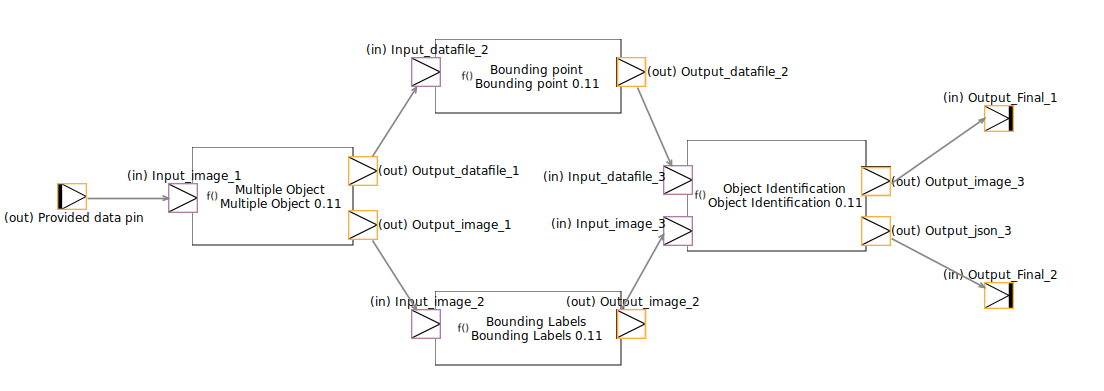
\includegraphics[width=0.95\linewidth]{./images/sirius-desktop-cal-example-model.png}
	\caption{Przykładowy diagram reprezentujący model EMF języka CAL w
		\emph{Sirius Desktop}.}\label{rys:sirius-desktop-cal-example-model}
\end{figure}
% \end{noindent}

Oprócz podstawowej struktury metamodelu oraz jego reprezentacji w formie
diagramu zostały do niego dodane dodatkowe funkcjonalności. Zostały one opisane
w kolejnych sekcjach.

\subsection{Warunkowa zmiana stylu elementów}

% \begin{noindent}
Użytkownik może wywnioskować dodatkowe informacje z diagramu jeżeli jego wygląd
będzie zależał od właściwości elementów modelu. Takie rozwiązanie zastosowano
dla dwóch elementów metamodelu dzięki wykorzystaniu \emph{Style
	Customizations}~\cite{sirius-desktop-documentation-style-customizations}
w \gls{EMF}.
% \end{noindent}
Funkcjonalność ta pozwala na wskazanie za pomocą języka \gls{AQL} w jakich
sytuacjach styl elementu powinien zostać zmieniony, a następnie wskazać które
właściwości powinny ulec zmianie oraz ich nowe wartości.

Pierwszy styl warunkowy został użyty dla portów w metamodelu. Porty
(\texttt{DataPin}) zmieniają ikonę na podstawie swoich krotności danych oraz
paczek danych (odpowiednio \emph{data multiplicity} i \emph{token
	multiplicity}).

Z uwagi na fakt, że oba parametry mogą mieć jedną z 2 wartości,
co daje w sumie 4~możliwości, w klasie \texttt{Services} metamodelu stworzono
metodę w języku Java, która zwraca nazwę odpowiedniej ikony.
Dzięki możliwości wykorzystania języka programowania osiągnięto
zamierzony efekt za pomocą jednego stylu warunkowego, a nie 4 różnych
styli dla 4 możliwości. Kod metody zwracającej nazwę ikony dla portu
został przedstawiony w listingu~\ref{lst:getDataPinIconPath-method}.

\begin{lstlisting}[float,
    floatplacement=ht,
    language=Java,
    caption={Methoda zwracająca nazwę ikony dla portu.},
    label={lst:getDataPinIconPath-method}]
public String getDataPinIconPath(EObject self) {
  if (!(self instanceof DataPin)) {
    return null;
  }

  var dataPin = (DataPin) self;
  var dataPart = dataPin.getDataMultiplicity() == Multiplicity.SINGLE ? "single-data" : "multiple-data";
  var tokenPart = dataPin.getTokenMultiplicity() == Multiplicity.SINGLE ? "single-token" : "multiple-tokens";

  return dataPart + "-" + tokenPart + ".png";
}
\end{lstlisting}

Dla portów całej aplikacji obliczeniowej (\texttt{ApplicationDataPin} dla
\texttt{Computation-\linebreak ApplicationRelease}) styl warunkowy był
rozszerzeniem tego
dla portów modułów obliczeniowych. Oprócz brania pod uwagę kroności danych oraz
paczek danych, w tym stylu znaczenie ma ponadto kierunek portu. Porty wejściowe
mają pogrubiony pasek z lewej strony, a porty wyjściowe z prawej. Dla tych
portów występują 3 cechy od których zależy ikona, co oznacza 8 możliwości.
Dzięki wykorzystaniu metody z listingu~\ref{lst:getDataPinIconPath-method} oraz
języka \gls{AQL} ta funkcjonalność została zrealizowana za pomocą jednego stylu
warunkowego, zamiast 8 styli dla 8 różnych wariantów.

Drugim wykorzystanym rodzajem styli warunkowych jest zmiana koloru obramowania
portów na krawędziach modułów obliczeniowych (\texttt{ComputedDataPin}) w
zależności od~kierunku przepływu danych. Porty wejściowe (\emph{required}) mają
ramkę koloru fioletowego, a~porty wyjściowe (\emph{provided}) mają ramkę koloru
pomarańczowego. Ta funkcjonalność została zaimplementowana za pomocą jednego
stylu warunkowego.

Wyniki działania obu rodzajów styli warunkowych widoczne są na
rysunku~\ref{rys:sirius-desktop-cal-example-model}.

\subsection{Narzędzia edytora diagramów}\label{sec:cal-metamodel-tools}

W metamodelach \gls{EMF} można zdefiniować narzędzia wspomagające i ułatwiające
edycję modeli, a także pomagające uniknąć
błędów~\cite{sirius-desktop-documentation-tools}. Również do metamodelu języka
CAL dodano takie narzędzia, które zostaną omówione w tej sekcji.

Pierwszą grupą narzędzi dodanych do metamodelu EMF języka CAL są narzędzia
automatyzujące pracę użytkownika, aby ten nie musiał manualnie wykonywać
niektórych czynności, a~jednocześnie aby w modelu nie znajdowały się nieużywane
elementy.

Jednym z takich narzędzi jest automatyczne usuwanie połączeń między portami
w~momencie, gdy ten port zostaje usunięty. W przypadku portów aplikacji
obliczeniowej (\texttt{ApplicationDataPin}) narzędzie to zastępuje zwykłą
operację usunięcia. Dla portów wywołania modułu obliczeniowego
(\texttt{ComputedDataPin}), narzędzie to uruchamiane jest podczas usuwania tego
modułu obliczeniowego. Dzięki temu narzędziu w modelu nie pozostają połączenia
zakończone jedynie z jednej strony.

Drugim z narzędzi automatyzujących pracę jest automatyczne zarządzanie
portami wywołania modułu obliczeniowego (\texttt{ComputedDataPin}) w~momencie
wskazania lub zmiany który moduł obliczeniowy ma zostać wywołany. Zmiana
atrybutu \texttt{unit} obiektu \texttt{UnitCall} usuwa aktualnie powiązane z
nim porty (o ile jakieś istniały) i tworzy nowe na podstawie definicji modułu
obliczeniowego (\texttt{ComputationUnitRelease}) zapisanej w metamodelu,
a~także jego zdeklarowanych portów (\texttt{DeclaredDataPin}). Stworzone porty
mają
automatycznie ustawione odwołania na właściwe deklaracje portów.
Wykorzystanie tego narzędzia zostało przedstawione na
rysunku~\ref{rys:sirius-desktop-change-unit-to-call}.

Narzędzie to zostało przygotowane poprzez modyfikację kodu źródłowego klas
metamodelu. Została zmieniona definicja metody zmiany wskazania na moduł do
wywołania w obiekcie \texttt{UnitCall}. Podczas wywołania tej metody usuwane są
poprzednie porty i tworzone są nowe. To zachowanie opisane jest w języku Java.

Dzięki temu narzędziu użytkownik nie musi samemu usuwać starych portów
i~tworzyć nowych podczas zmiany wywoływanego modułu. Przyśpiesza to~pracę z
metamodelem i~pomaga uniknąć błędów.

% \begin{noindent}
\begin{figure}
	\centering
	\begin{subfigure}{.3\textwidth}
		\centering
		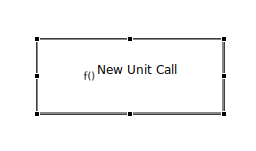
\includegraphics[width=.99\linewidth]{./images/sirius-desktop-empty-unit-call.png}
		\caption{Nowo utworzone wywołanie modułu obliczeniowego.}\label{ref:sirius-desktop-empty-unit-call}
    \medskip
    {\small To wywolanie nie~ma~wskazanego modułu, które ma wywołać, stąd
      druga linia etykiety jest pusta.}
    \vspace{50pt}
	\end{subfigure}
	\begin{subfigure}{.3\textwidth}
		\centering
		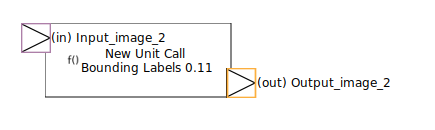
\includegraphics[width=.99\linewidth]{./images/sirius-desktop-change-unit-to-call-before.png}
		\caption{Wywołanie modułu obliczeniowego po wskazaniu modułu do wywołania.}\label{
      rys:sirius-desktop-change-unit-to-call-before}
    \medskip
    {\small Porty zostały automatycznie utworzone zgodnie z~deklaracją modułu
      \emph{Bounding Labels}.}
    \medskip
	\end{subfigure}
	\begin{subfigure}{.3\textwidth}
		\centering
		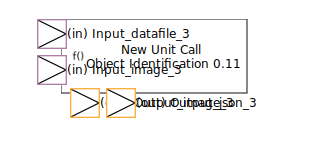
\includegraphics[width=.99\linewidth]{./images/sirius-desktop-change-unit-to-call-after.png}
		\caption{Wywołanie modułu obliczeniowego po ponownym wskazaniu modułu do wywołania.}\label{
      rys:sirius-desktop-change-unit-to-call-after}
    \medskip
    {\small Poprzednie porty zostały usunięte, a na ich miejsce zostały
      utworzone nowe, bazując na zdeklarowanych portach modułu \emph{Object
      Identification}.}
	\end{subfigure}

	\caption{Demonstracja działania narzędzia zarządzającego portami wywołań
    modułów obliczeniowych.}\label{rys:sirius-desktop-change-unit-to-call}
\end{figure}
% \end{noindent}

Inną grupą narzędzi są narzędzia pomagające w przestrzeganiu poprawności
modelu. Do~tej~grupy można zaliczyć kilka narzędzi dotyczących tworzenia lub
modyfikacji połączeń między portami. Dane mogą przepływać jedynie od portów
wyjściowych do portów wejściowych. Ponadto, niemożliwe jest połączenie portów
na tym samym wywołaniu modułu obliczeniowego. Oba te wymagania mogą być
egzekwowane w modelu za pomocą narzędzi do tworzenia połączeń (\emph{Edge
	Creation}) oraz do zmiany połączenia (\emph{Reconnect Edge}). Pierwsze
z nich za
pomocą warunków \emph{Connection Start Precondition} oraz
\emph{Connection Complete Precondition}, ustalających czy połączenie może
zostać
rozpoczęte lub zakończone w~danym elemencie, pozwala zabronić stworzenia
połączenia. Drugie z nich za pomocą warunku \emph{Precondition} ustala kiedy
zmiana jednego z końców połączenia jest możliwa.

Drugim z narzędzi w grupie pomagających w przestrzeganiu poprawności jest
narzędzie uniemożliwiające usuwanie portów wywołań modułów obliczeniowych
(\texttt{ComputedDataPin}). Są one tworzone i usuwane automatycznie podczas
wskazania modułu do wywołania i~niepoprawnym byłoby gdyby użytkownik mógł
tworzyć lub usuwać je samemu, ponieważ faktyczna liczba portów mogłaby się
wtedy nie
zgadzać z liczbą zadeklarowanych portów w~tym~module obliczeniowym.

Innym typem narzędzi są narzędzia ułatwiające tworzenie elementów modelu.
Są~3~proste narzędzia umieszczających element w modelu: dla portu wejściowego i
wyjściowego aplikacji, a także dla pustego wywołania modułu obliczeniowego, dla
którego należy później wskazać moduł, który ma wywołać. Bardziej skomplikowanym
narzędziem jest narzędzie pozwalające na~dodanie do modelu wywołania modułu
obliczeniowego, które pokazuje okno dialogowe pozwalające wybrać moduł oraz
wskazać nazwę dodawanego obiektu. Wykorzystuje ono~możliwości \emph{Sirius
	Desktop} do tworzenia okien dialogowych (zarówno jednorazowych
jak~i~składających się z wielu
kroków)~\cite{sirius-desktop-documentation-tools} i
pozwala na dostarczeniu użytkownikowi
bardziej interaktywnych i przyjemniejszych wrażeń z pracy z modelem. Okno
dialogowe
pokazujące się po wybraniu
tego narzędzia jest przedstawione na
rysunku~\ref{rys:sirius-desktop-create-unit-call-tool}.

% \begin{noindent}
\begin{figure}[!hb]
	\centering

	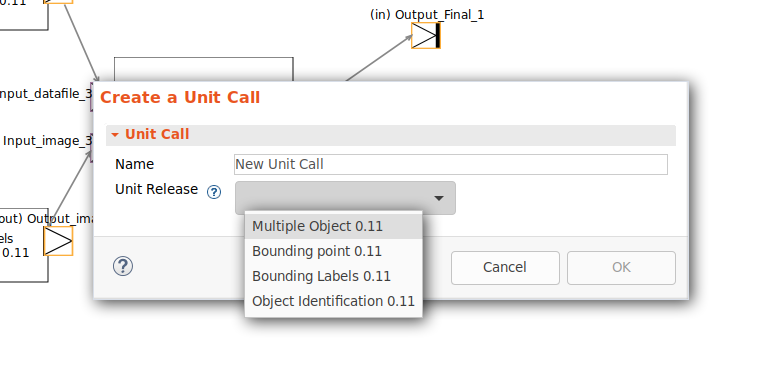
\includegraphics[width=0.95\linewidth]{./images/sirius-desktop-create-unit-call-tool.png}
	\caption{Narzędzie do interaktywnego tworzenia nowego wywołania modułu
		obliczeniowego w~\emph{Sirius Desktop}.}\label{rys:sirius-desktop-create-unit-call-tool}
\end{figure}
% \end{noindent}

Narzędzia te uruchamiają się jedynie, gdy zmiana w modelu zostanie wykonana
poprzez edycję diagramu lub właściwości już istniejącego elementu. Podczas
bezpośredniej edycji drzewa modelu narzędzia powiązane z metamodelem są
pomijane, przez co można doprowadzić do sytuacji, w której model nie będzie
poprawny
semantycznie. Przykładem operacji pomijającej narzędzia jest usunięcie portu
aplikacji obliczeniowej (\texttt{ApplicationDataPin}) bezpośrednio z~drzewa
modelu. Jeżeli miała ona połączenie (\texttt{DataFlow}), nie zostanie ono
automatycznie usunięte (narzędzie, które je usuwa nie zostanie uruchomione), co
prowadzi do istnienia w~modelu połączenia, którego jedynie jeden koniec jest
poprawnie ustawiony. Takie sytuacje natomiast są wykrywane przez reguły
walidacji strukturalnej metamodelu (połączenie musi mieć poprawne oba końce).

\subsection{Reguły walidacyjne powiązane z
	metamodelem}\label{sec:reguly-walidacyjne-metamodel}

\emph{Sirius Desktop} dostarcza mechanizm walidacji edytowanego modelu. Można
go uruchomić poprzez wybranie opcji \menu{Diagram > Validate} z głównego menu
programu. Wyświetlona zostanie wtedy lista informacji diagnostycznych
dotyczących modelu.

\emph{Sirius Desktop} domyślnie dostarcza informacji o błędach składniowych
modelu. Będą to~ostrzeżenia o braku wymaganych atrybutów lub niepoprawnej
krotności elementow (jeżeli dana właściwość powinna zawierać przykładowo co
najmniej 3 elementy, a nie więcej niż~5~elementów). Błędy te będą także
zaznaczone na diagramie za pomocą ikony czerwonego znaku \texttt{X} obok
elementu, którego wiadomość dotyczy. Zostało to zilustrowane na
rysunku~\ref{rys:sirius-desktop-syntax-validation}.

% \begin{noindent}
\begin{figure}[!hb]
	\centering

	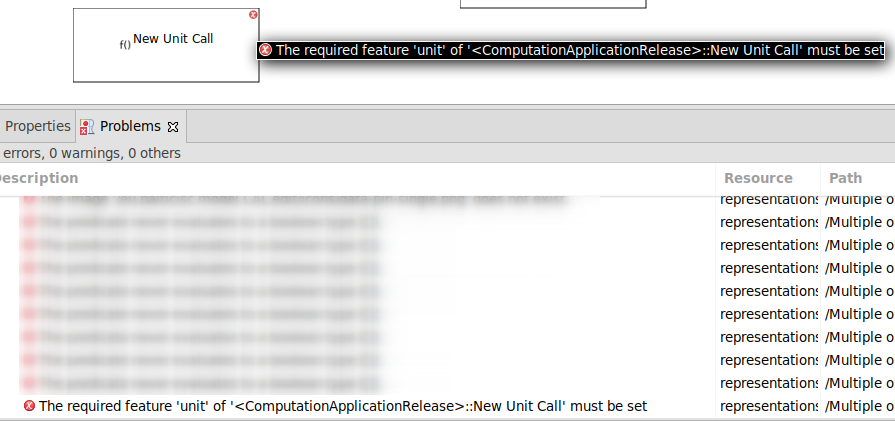
\includegraphics[width=0.95\linewidth]{./images/sirius-desktop-syntax-validation.png}
	\caption{Walidacja składniowa modeli w \emph{Sirius
  Desktop}.}\label{rys:sirius-desktop-syntax-validation}
\end{figure}
% \end{noindent}

Dodatkowo w pliku \texttt{*.odesign} pakietu \texttt{.design} metamodelu można
zdefiniować \emph{Semantic Validation
	Rules}~\cite{sirius-desktop-documentation-validation-rules}.
Pozwalają one na dodanie własnych reguł walidacji semantycznej modeli. To
reguły powinny opisywać ograniczenia, których nie dostarcza opis strukury
modelu i~zależą od połączenia kilku elementów ze sobą. Można
wybrać jakich elementów reguła dotyczy, a~za~pomocą języka \gls{AQL} wskazać
kiedy informacja diagnostyczna powinna być pokazana, a także jaka powinna być
wiadomość wyświetlona użytkownikowi, oraz z jakim poziomem poważności
(informacja, ostrzeżenie, błąd). Jeżeli wiadomo jak można naprawić błąd, można
zdefiniować również sekwencję akcji, które będą wykonywane gdy użytkownik
wybierze
opcje automatycznego naprawiania błędów diagnostycznych.

Przykładową regułę walidacji semantycznej przedstawiono na
rysunku~\ref{rys:sirius-desktop-example-semantic-validation-rule}.
Zabrania ona~połączeń między portami znajdującymi się na tym samym wywołaniu
modułu obliczeniowego. Jej struktura wyrażona w drzewie obiektów metamodelu
jest widoczna na
rysunku~\ref{rys:sirius-desktop-example-semantic-validation-rule-tree}, a jej
właściwości na
rysunku~\ref{rys:sirius-desktop-example-semantic-validation-rule-properties}.
Widać tam element, dla którego wiadomość zostanie wyświetlona
(\texttt{DataFlow}).
Rysunek~\ref{rys:sirius-desktop-example-semantic-validation-rule-audit}
przedstawia wyrażenie języka \gls{AQL}. Niespełnienie warunku spowoduje
pokazanie
informacji o błędzie. W tym przypadku sprawdza ono, czy~obiekty początkowy i
końcowy połączenia mają różnych rodziców. Nie jest to spełnione wyłącznie
jeżeli oba~porty należą do tego samego wywołania modułu obliczeniowego.
Błąd wynikający z tej reguły został
przedstawiony na
rysunku~\ref{rys:sirius-desktop-example-semantic-validation-rule-failure}.
Należało wykluczyć sytuacje, w
których połączenie jest między dwoma portami aplikacji obliczeniowej, ponieważ
takie połączenia są dozwolone.

% \begin{noindent}
\begin{figure}
	\centering
	\begin{subfigure}{.8\textwidth}
		\centering
		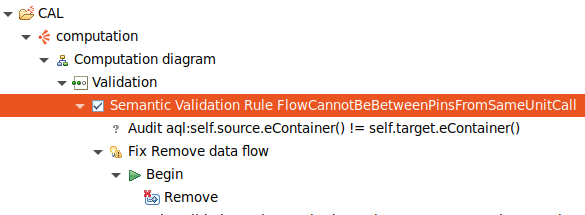
\includegraphics[width=.99\linewidth]{./images/sirius-desktop-example-semantic-validation-rule-tree.png}
		\caption{Drzewo obiektów składających się na regułę walidacji
      semantycznej.}\label{rys:sirius-desktop-example-semantic-validation-rule-tree}
	\end{subfigure}

  \medskip

	\begin{subfigure}{.92\textwidth}
		\centering
		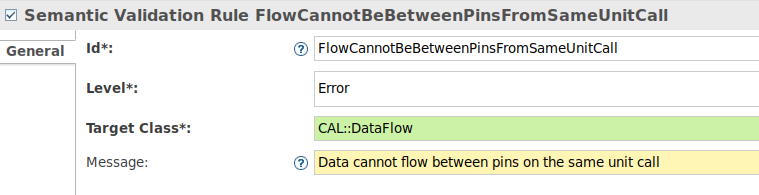
\includegraphics[width=.99\linewidth]{./images/sirius-desktop-example-semantic-validation-rule-properties.png}
		\caption{Właściwości reguły walidacji semantycznej.}\label{rys:sirius-desktop-example-semantic-validation-rule-properties}
	\end{subfigure}

  \medskip

	\begin{subfigure}{.92\textwidth}
		\centering
		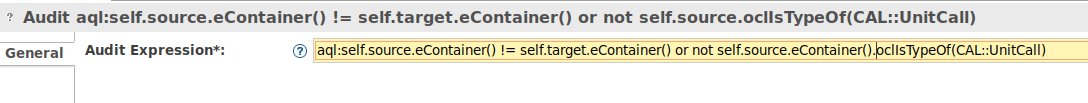
\includegraphics[width=.99\linewidth]{./images/sirius-desktop-example-semantic-validation-rule-audit.png}
		\caption{Warunek spełnienia reguły walidacji semantycznej.}\label{rys:sirius-desktop-example-semantic-validation-rule-audit}
	\end{subfigure}

  \begin{subfigure}{.92\textwidth}
    \centering
    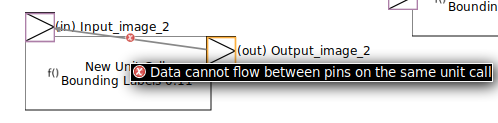
\includegraphics[width=.99\linewidth]{./images/sirius-desktop-example-semantic-validation-rule-failure.png}
    \caption{Błąd --- reguła nie została
    spełniona.}\label{rys:sirius-desktop-example-semantic-validation-rule-failure}
  \end{subfigure}

	\caption{Przykładowa reguła walidacji semantycznej w \emph{Sirius
  Desktop}.}\label{rys:sirius-desktop-example-semantic-validation-rule}
  \medskip
  {\small Reguła zabrania występowania połączeń między portami na tym samym
  wywołaniu modułu obliczeniowego.}
\end{figure}
% \end{noindent}

Oprócz reguły walidacji semantycznej zaprezentowanej na
rysunku~\ref{rys:sirius-desktop-example-semantic-validation-rule}
zaprojektowano 5~innych reguł informujących użytkownika o błędach w metamodelu.
Pierwsze dwie z~nich pomagają ustalić oczekiwany kierunek połączeń portów. Dla
portów oznaczonych jako wymagane (\texttt{required}) połączenie powinno być
wchodzące, a dla portów oznaczonych jako dostarczone (\texttt{provided}) ---
wychodzące. Jest to informacja niewynikająca ze struktury metamodelu, więc
została dostarczona jako reguła walidacji semantycznej. Oprócz 2 reguł
wymagających połączenia danego typu są też 2 reguły, które zabraniają
połączenia w~przeciwną stronę niż oczekiwana. Oznacza to, że jeżeli port nie
będzie miał żadnego połączenia, będzie pokazana informacja o braku, a jeżeli
dodatkowo port będzie miał połączenie w~przeciwną stronę (przykładowo, port
wymagany będzie miał połączenie wychodzące), to będą 2~wiadomości: jedna o
braku połączenia w oczekiwanym kierunku, a druga o~nieoczkiewanym połączeniu w
przeciwnym kierunku.

Ostatnią dodaną regułą jest sprawdzenie czy oba końce połączenia (obiektu
\texttt{DataFlow}) są~zdefiniowane. Jeżeli krawędź nie jest połączona z dwoma
obiektami, użytkownik dostaje o tym informacje oraz możliwość szybkiego
usunięcia takiego połączenia. Jest to szczególnie ważne, ponieważ takie
połączenia nie są pokazywane na diagramie, a jedynie wprowadzają zamieszanie w
metamodelu i utrudniają badanie jego struktury przez narzędzia, które muszą
oczekiwać, że krawędzie mogą nie być zaczepione z obu stron.

\subsection{Testy metamodelu}\label{sec:testy-metamodelu}

W sekcji~\ref{sec:cal-metamodel-tools} opisano modyfikacje kodu źródłowego klas
metamodelu, które usprawniają pracę użytkownika z modelem. Aby upewnić się, że
te modyfikacje działają poprawnie, należy je~przetestować. Można to zrobić
projektując testy
jednostkowe metamodelu w pakiecie \texttt{.tests}. \emph{Sirius Desktop}
automatycznie generuje kod źródłowy posiadający odpowiednią strukturę do
tworzenia testów. Dla każdego obiektu metamodelu tworzona jest osobna klasa z
jego testami.

Oprócz zwykłych plików z testami wygenerowane zostały również pliki dla
pakietów testów (\emph{\selectlanguage{english}test suite}), w których można
zdefiniować grupy testów,
które mają zostać wykonane. W~ten~sposób można podzielić testów na kilka
kategorii, na przykład testy krytyczne, testy normalne, testy o niskiej
ważności. Zgrupowanie testów pozwala na otrzymanie podsumowanego statusu
wszystkich testów w danej grupie.

Testy można później w łatwy i szybki sposób uruchomić zaznaczając pakiet z
testami w eksploratorze projektów, a później wybierając z menu głównego
\menu{Run > Run As > JUnit Test}. Uruchamiane są one wykorzystując popularny
zestaw narzędzi \emph{JUnit}~\cite{junit-test-tutorial}.

Posiadanie testów jednostkowych pozwala w szybszy sposób sprawdzić czy model
nadal zachowuje się zgodnie z oczekiwaniami, co jest szczególnie ważne po
modyfikacji jego kodu źródłowego lub generowaniu go na nowo po zmianach
metamodelu. Należy testować kod~zmodyfikowany lub dodany. Nie należy testować
kodu automatycznie generowanego przez \emph{Sirius Desktop} jeżeli nie został
on zmodyfikowany.

W ramach tej pracy magisterskiej przygotowano 2 testy jednostkowe weryfikujące
następujące zachowania dodane w kodzie źródłowym klas metamodelu:

\begin{itemize}
	\item Czy połączenia między portami usuwanych wywołań węzłów obliczeniowych są również usuwane?

	\item Czy porty są automatycznie usuwane i tworzone podczas zmiany wskazania modułu, który ma zostać wywołany w danym obiekcie \texttt{UnitCall}?

	      Weryfikowane jest czy utworzone porty mają poprawnie ustawione odwołania na~zdeklarowane porty danego modułu obliczeniowego.
\end{itemize}

Są to jedyne dwie modyfikacje kodu źródłowego metamodelu, których dokonano.
Wyniki uruchomienia testów jednostkowych przedstawione są na
rysunku~\ref{rys:sirius-desktop-metamodel-tests}. Wszystkie zdefiniowane testy
zakończyły się powodzeniem. Interfejs pokazuje 6 niepowodzeń (\emph{failures}),
ponieważ z~7~wygenerowanych plików z testami (po jednym dla każdego obiektu
metamodelu), tylko jeden ma zdefiniowane w sobie testy, a reszta jest pusta.
Niepowodzenie informuje o braku testów zdefiniowanych w tych plikach.

W przypadku tego metamodelu są przygotowane
jedynie dwa testy, więc nie było potrzeby dzielić je na grupy
(\emph{\selectlanguage{english}test suites}) --- jest tylko
jedna grupa nadrzędna \emph{\selectlanguage{english}CAL All Tests}, która
zawiera w sobie grupę
\emph{\selectlanguage{english}CAL Tests}, która zawiera poszczególne testy.

% \begin{noindent}
\begin{figure}[!hb]
	\centering

	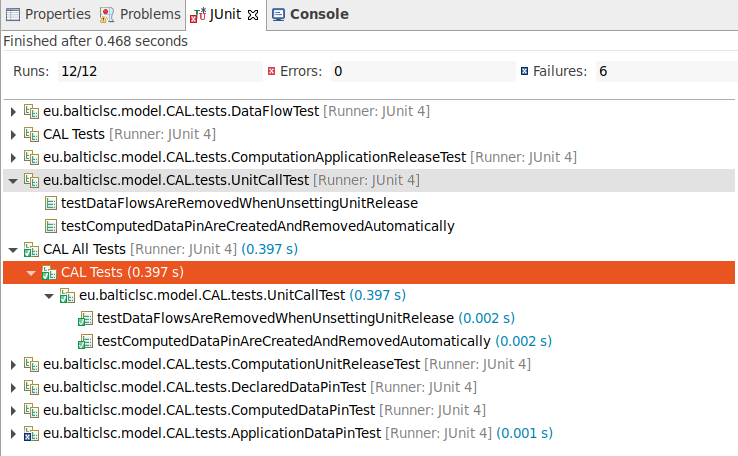
\includegraphics[width=0.95\linewidth]{./images/sirius-desktop-metamodel-tests.png}
	\caption{Wynik uruchomienia testów automatycznych
  metamodelu.}\label{rys:sirius-desktop-metamodel-tests}
\end{figure}
% \end{noindent}


\chapter{Dostosowanie Sirius Web dla systemu BalticLSC}

\section{Użycie metamodelu języka CAL w Sirius Web}

Opis jak wykorzystać metamodel EMF w Sirius Web.

\begin{itemize}
	\item konfiguracja Maven
	\item odpowiednia modyfikacja klas Javy w Sirius Web
\end{itemize}

\noindent oraz jaki rezultat uzyskano.

\section{Integracja przybornika BalticLSC w Sirius Web}

Opis problemu dodawania nowych \texttt{UnitCall} do diagramu --- trzeba
zdefiniować \texttt{ComputationUnitRelease} w diagramie.

Rozwiązanie (zaczerpnięte z edytora diagramów BalticLSC) --- przybornik
(toolbox).

Opis jak to zrobiono, od strony backendu jak i frontendu. Omówienie trudności w
modyfikacji interfejsu użytkownika Sirius Web (trzeba było skopiować kod
źródłowy niektórych komponentów z biblioteki \textit{Sirius Components} do kodu
aplikacji Sirius Web, ponieważ komponenty te nie umożliwiały modyfikacji
interfejsu i wstawiania do nich nowych elementów --- najlepiej dać zrzut ekranu
co można było łatwo zmienić, a co wymagało skopiowania kodu).

\section{Walidacja semantyczna modelu}

Informacja o informacjach diagnostycznych udostępnianych domyślnie przez Sirius
Web.

Brak uruchamiania reguł semantycznych zdefiniowanych w
metamodelu~\ref{sec:reguly-walidacyjne-metamodel}.

Opis dodanego rozwiązania (własne klasy Javowe które zwracają listę informacji
diagnostycznych, oraz strumieniowanie ich do przeglądarki wykorzystując
istniejące rozwiązanie do walidacji).

\section{Użycie edytora Sirius Web w BalticLSC}

Omówienie przygotowanego planu integracji.

\chapter{Ocena Sirius Web}

\section{Różnice między Sirius Web a Sirius Desktop}

Omówienie różnic oraz usterek zgłoszonych przeze mnie w repozytorium Sirius
Web.

\section{Użycie własnego metamodelu}

\section{Dodawanie funkcjonalności do edytora}

\chapter{Informacje techniczne}

\section{Wykorzystane biblioteki}

Tabela z wykorzystywanymi bibliotekami i ich licencjami.

\section{Projekt systemu}

Diagram z backendami oraz frontendami BalticLSC, a także bazą danych
PostgreSQL\@.

\section{Projekt modułów}

Informacje o modułach backendu (projekty Javy w Sirius Web).

\section{Instrukcja wdrożenia}

\subsection{Wymagania}

Docker, lub Java 11, Maven, PostgreSQL

\subsection{Instrukcja instalacji}

Opis: albo Docker, albo instalacja manualna (potwórzenie instrukcji z
\texttt{README.md}).

\subsection{Instrukcja uruchomienia}

Opis: albo Docker, albo manualnie uruchomienie serwera

\section{Instrukcja użycia}

Jak użyć aplikacji do stworzenia prostego modelu

Powinno także zawierać informacje o logowaniu się do BalticLSC\@.

\section{Instrukcja utrzymania}

\subsection{Kopia zapasowa bazy danych}

Jak stworzyć kopię bazy w PostgreSQL\@?

\subsection{Aktualizowanie wersji Sirius Web}

Opis metody aplikowania najnowszych zmian z repozytorium Sirius Web
(generowanie \texttt{git patch} i aplikowanie ich).

\section{Zabezpieczenia}

Brak zabezpieczeń.

\section{Testy akceptacyjne rozwiązania}

Opis kilku testów, które użytkownik może chcieć wykonać aby sprawdzić, czy
rozwiązanie działa poprawnie.

\subsection{Wynik testów akceptacyjnych}

Czy się udały?

\chapter{Podsumowanie}

\section{Wyniki pracy}

Co zostało osiągnięte? Czy cel został zdobyty?

\section{Wnioski}

Sirius Web jest w fazie rozwoju, ale można już go użyć. Brakuje dokumentacji,
więc wymagany jest \textit{reverse engineering}, czytanie kodu źródłowego,
metoda prób i błędów, debuggowanie aplikacji, zgłaszanie usterek lub zadawanie
pytań w repozytorium projektu.

Występują różnice między Sirius Web a Sirius Desktop.

\section{Możliwości na rozwój}

Wymienić co można zrobić dalej:

\begin{itemize}
	\item integracja z BalticLSC
	\item dodanie większej liczby reguł walidacji semantycznej
\end{itemize}
